\documentclass{article}
\usepackage{graphicx} % Required for inserting images
\usepackage[polish]{babel}
\usepackage{minted}
\usepackage[letterpaper,top=2cm,bottom=2cm,left=3cm,right=3cm,marginparwidth=1.75cm]{geometry}
\usepackage{amsmath}
\usepackage{graphicx}
\usepackage[colorlinks=true, allcolors=blue]{hyperref}
\usepackage[T1]{fontenc}
\usepackage[table,xcdraw]{xcolor}
\makeatletter
\renewcommand{\paragraph}{\@startsection{paragraph}{4}{0ex}%
   {-3.25ex plus -1ex minus -0.2ex}%
   {1.5ex plus 0.2ex}%
   {\normalfont\normalsize\bfseries}}
\makeatother

\title{MOwNiT - Porównanie metod interpolacji i aproksymacji dla zadanej funkcji}
\author{Jakub Frączek}
\date{April 2024}

\begin{document}

\maketitle

\section{Dane techniczne}

\subsection{Hardware}

Laptop z procesorem Intel Core i5-9300H 2.4GHz oraz 32 GB pamięci RAM.

\subsection{Software}

Wykorzystany został system Windows 11 x64 oraz język Python w wersji 3.11.8 wraz z bibliotekami:
\begin{itemize}
\item math
\item copy
\item matplotlib
\item numpy
\end{itemize}

\section{Funkcja dla której przeprowadzone zostało doświadczenie}

\begin{center}
\(f(x) = 10 * m + \frac{\mathrm{x}_{}^{2}}{k} - 10 * m * cos(k*x)\)
\end{center}

\noindent
gdzie:

\bigbreak

\(k = 1.5\)
\newline \indent
\(m = 3.0\)
\newline \indent
\(x \in [-4\pi, 4\pi]\)

\bigbreak

Wykres funkcji:

\begin{figure}[H]
  \centering
  \begin{minipage}[b]{0.5\textwidth}
    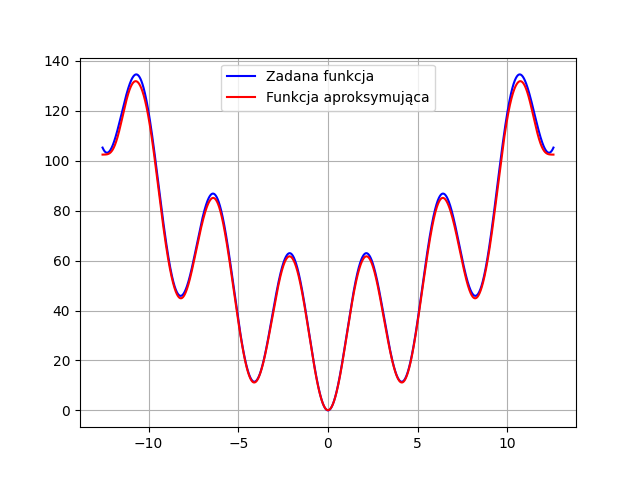
\includegraphics[width=\textwidth]{zadana_funkcja.png}
  \end{minipage}
\end{figure}

\newpage

\section{Własności funkcji w zadanym przedziale}

\begin{itemize}
    \item Symetryczna względem osi OY
    \item Liczne oscylacje
    \item Znaczne skoki wartości funkcji na krańcach przedziałów
\end{itemize}

\section{Metody przyblizania funkcji}

Poniżej opisane są metody, które zostały wykorzystane do przybliżania funkcji.

\subsection{Interpolacja}

Jest to metoda, która polega na wyznaczeniu funkcji interpolującej, która w danym przedziale przyjmuje ustalone wartości w z góry zadanych punktach. Funkcja interpolująca może być wielomianem algebraicznym lub składać się z kilku funkcji.

\bigbreak

W szczególności wykorzystane zostały:

\begin{itemize}
    \item Interpolacja Lagrange'a
    \item Interpolacja Newtona
    \item Interpolacja Hermite'a
    \item Interpolacja funkcją sklejaną 2-go stopnia z warunkami brzegowymi:
    \begin{itemize}
        \item Natural boundary
        \item Clmaped boundary
    \end{itemize}
    \item Interpolacja funkcją sklejaną 3-go stopnia z warunkami brzegowymi:
    \begin{itemize}
        \item Default boundary
        \item Natural boundary
    \end{itemize}
\end{itemize}

\subsection{Aproksymacja}

Polega na znalezieniu funkcji aproksymującej, która nie przechodzi przez wszystkie zadane punkty (tak jak było w interpolacji), tylko odzwierciedla ogólny trend w danych, tj. czasem przechodzi pomiędzy węzłami, tak by jak najlepiej dopasować się do funkcji.

\bigbreak

W szczególności wykorzystane zostały:

\begin{itemize}
    \item Aproksymacja średniokwadratowa wielomianami algebraicznymi
    \item Aproksymacja średniokwadratowa wielomianami trygonometrycznymi
\end{itemize}

\section{Analiza}

W poniższych podpunktach opisane zostały problemy występująće dla danego typu przybliżenia ze względu na charakter funkcji.
\bigbreak
\noindent
Sposoby liczenia błędów

\begin{center}
    \(\max_{x\in [a, b]} |F(x) - \mathrm{P}_{n}^{}(x)|\)
\end{center}

\begin{center}
\(\frac{1}{N} * \sum_{i = 1}^{N}\mathrm{(F(\mathrm{x}_{i}^{}) - \mathrm{P}_{n}^{}(\mathrm{x}_{i}^{}))}_{}^{2}\)
\end{center}

\newpage

\subsection{Interpolacja Lagrange'a}

\subsubsection{Opis teoretyczny}

Wielomian interpolacyjny Lagrange'a można wyrazić wzorem:
\[\sum_{k=0}^{n} f(\mathrm{x}_{k}^{})\mathrm{L}_{k}^{}\]
gdzie:
\bigbreak
\( f(\mathrm{x}_{k}^{})\ -\ wartości\ funkcji\ w\ punktach\ \mathrm{x}_{k}^{} \)
\bigbreak
\( \mathrm{L}_{k}^{}(x) = \frac{d}{m} = \prod_{i\ =\ 0, i\ !=\ k}^{n}\ \frac{x -\mathrm{x}_{i}^{}}{\mathrm{x}_{k}^{} - \mathrm{x}_{i}^{}}\ - \ baza\ Lagrange'a\)

\subsubsection{Napotkane trudności}

Pierwsza napotkana trudność przy interpolacji bezpośrednio wynika z dużych oscylacji funkcji, jak widać na poniższych wykresach węzły ułożyły się tak, że przybliżenie jest bardzo złe właśnie w wyniku oscylacji funkcji. Ta sytuacja zachodzi zarówno jak i dla równoodległych węzłów, jak i węzłów Czebyszewa.

\begin{figure}[H]
  \begin{minipage}[b]{0.49\textwidth}
    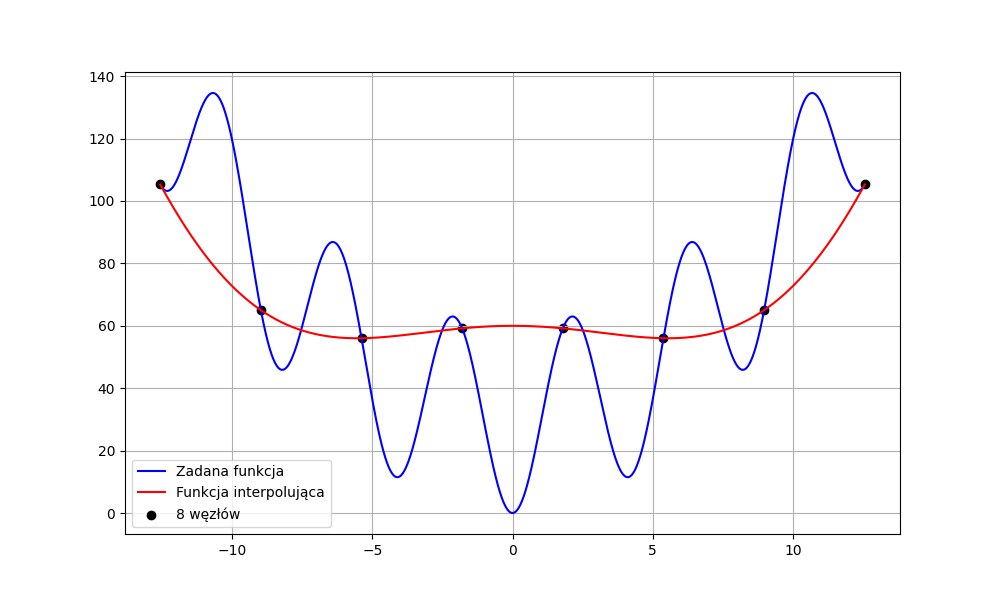
\includegraphics[width=\textwidth]{img01__n=8.png}
    \caption{Wykres dla 8 równoodległych węzłów}
  \end{minipage}
  \hfill
  \begin{minipage}[b]{0.49\textwidth}
    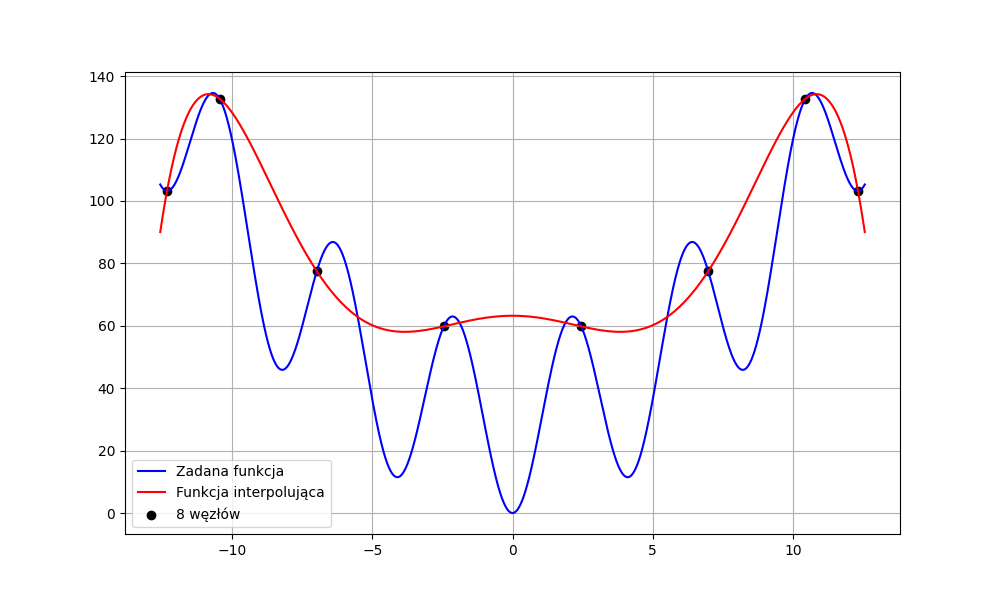
\includegraphics[width=\textwidth]{img02__n=8.png}
    \caption{Wykres dla 8 węzłów Czebyszewa}
  \end{minipage}
\end{figure}

Ten problem dobrze widać, też na przykładzie większej liczby węzłów Czebyszewa. Ponieważ jest ich więcej na krańcach przedziałów to przybliżenie jest tam dobre, a z uwagi na ich mniejszą ilość w środku 
znaczna oscylacja funkcji powoduje problemy z przybliżeniem właśnie w środku przedziału.

\begin{figure}[H]
\centering
  \begin{minipage}[b]{0.49\textwidth}
    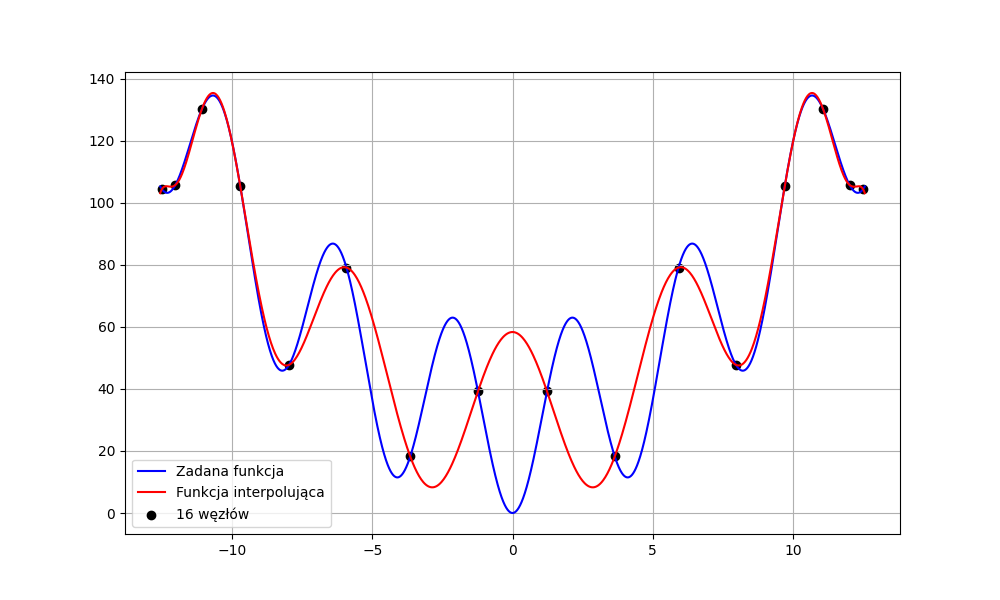
\includegraphics[width=\textwidth]{img02__n=16.png}
    \caption{Wykres dla 16 węzłów Czebyszewa}
  \end{minipage}
\end{figure}

\newpage

Kolejnym problemem była znaczna zmiana w wartościach funkcji na krańcach przedziałów, która powodowała problemy z przybliżeniem właśnie w okolicy, w której zachodziła ta szybka zmiana wartości, z tego powodu zdarzało się, że przybliżenie "wybiegało" znacznie poza funkcję, ta sytuacja została zaprezentowana poniżej.

\begin{figure}[H]
\centering
  \begin{minipage}[b]{0.49\textwidth}
    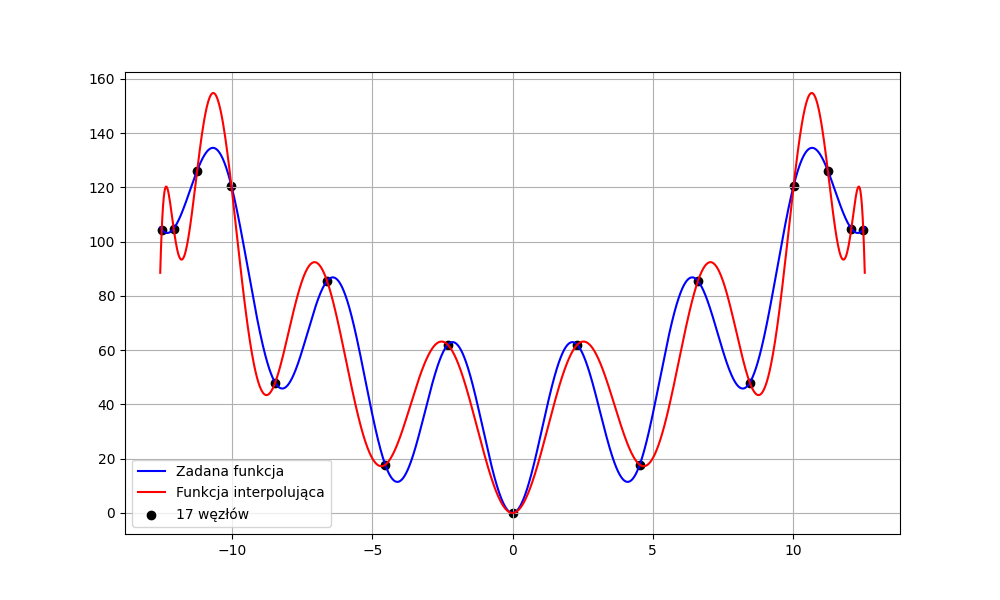
\includegraphics[width=\textwidth]{img02__n=17.png}
    \caption{Wykres dla 17 węzłów Czebyszewa}
  \end{minipage}
\end{figure}

\subsubsection{Najlepsze otrzymane przybliżenie}

Najlepsze przybliżenie ze względu na błąd maksymalny (dla 50 węzłów) oraz średniokwadratowy (dla 54 węzłów), można otrzymać korzystając jedynie z generacji węzłów zgodnie z zerami wielomianu Czebyszewa, a wartości błędów są dużo mniejsze niż w przypadku węzłów równoodległych.

\begin{figure}[H]
  \begin{minipage}[b]{0.49\textwidth}
    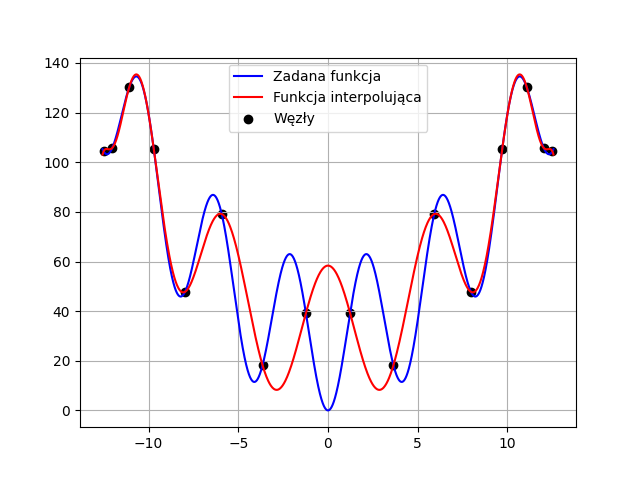
\includegraphics[width=\textwidth]{img03.png}
    \caption{Najlepsze przybliżenie ze względu na błąd maksymalny}
  \end{minipage}
  \hfill
  \begin{minipage}[b]{0.49\textwidth}
    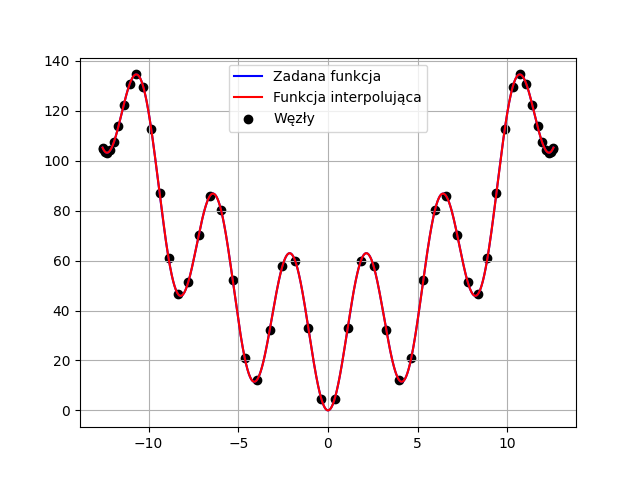
\includegraphics[width=\textwidth]{img04.png}
    \caption{Najlepsze przybliżenie ze względu na błąd średniokwadratowy}
  \end{minipage}
\end{figure}

Na poniższych wykresach są podane wartości błędów dla powyższych wykresów.

\begin{table}[!ht]
    \centering
    \begin{tabular}{|l|l|}
    \hline
        Błąd maksymalny & 1.9895196601282805e-13 \\ \hline
        Błąd średniokwadratowy & 2.296897441475515e-27 \\ \hline
    \end{tabular}
    \caption{Wartości błędów}
\end{table}

\newpage

\subsection{Interpolacja Newtona}

\subsubsection{Opis teoretyczny}

\[ \mathrm{P}_{n}^{}(x) = f[\mathrm{x}_{0}^{}] + \sum_{i = 1}^{n}f[\mathrm{x}_{0}^{}, \mathrm{x}_{1}^{}, ..., \mathrm{x}_{i}^{}]*(x - \mathrm{x}_{0}^{})*(x - \mathrm{x}_{1}^{})*...*(\mathrm{x}_{i - 1}^{})\]

\noindent
gdzie:
\bigbreak

\( f[\mathrm{x}_{i}^{}] = f(\mathrm{x}_{i}^{}) \) \newline \indent
\( f[\mathrm{x}_{i}^{}, \mathrm{x}_{i+1}^{}] = \frac{f[\mathrm{x}_{i+1}^{}]-f[\mathrm{x}_{i}^{}]}{\mathrm{x}_{i+1}^{}-\mathrm{x}_{i}^{}} \) \newline \indent
\( . \) \newline \indent
\( . \) \newline \indent
\( . \) \newline \indent
\( f[\mathrm{x}_{i}^{}, \mathrm{x}_{i+1}^{}, ..., \mathrm{x}_{i + k}^{}] =
\frac{f[\mathrm{x}_{i+1}^{}, \mathrm{x}_{i+2}^{}, ..., \mathrm{x}_{i + k}^{}] - f[\mathrm{x}_{i}^{}, \mathrm{x}_{i+1}^{}, ..., \mathrm{x}_{i + k -1}^{}]}{\mathrm{x}_{i+k}^{} - \mathrm{x}_{i}^{}} \) \newline

\subsubsection{Napotkane trudności}

Podobnie jak w przypadku interpolacji lagrange'a duża oscylacja wartości funkcji prowadzi do sytuacji, gdzie przybliżenie jest bardzo złe i przypomina linię prostą. To samo zachodzi zarówno dla równoodległych węzłów, jak i węzłów Czebyszewa. Ta sytuacja została pokazana poniże.

\begin{figure}[H]
  \begin{minipage}[b]{0.49\textwidth}
    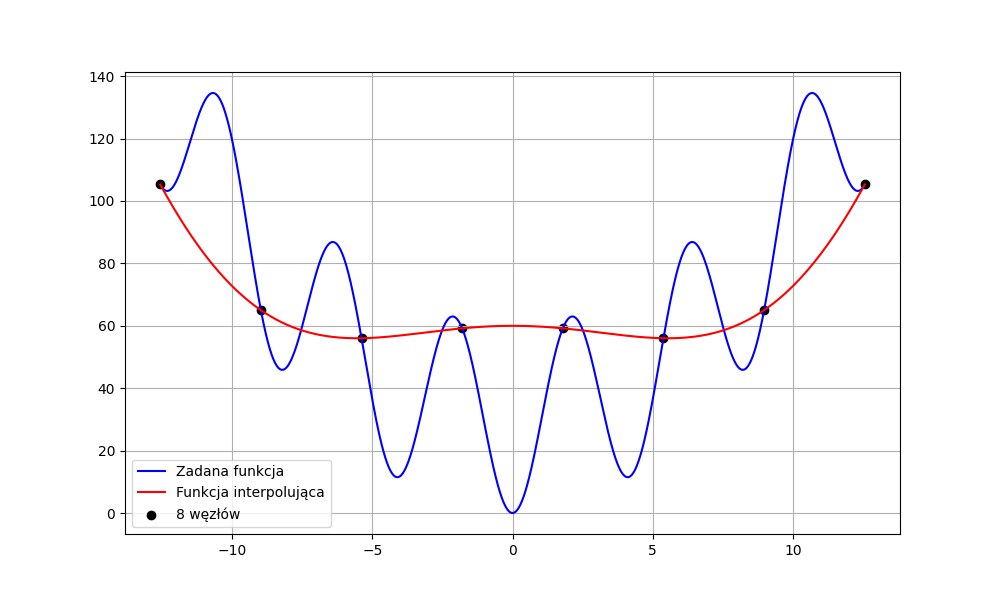
\includegraphics[width=\textwidth]{img05_n=8.png}
    \caption{Wykres dla 8 równoodległych węzłów}
  \end{minipage}
  \hfill
  \begin{minipage}[b]{0.49\textwidth}
    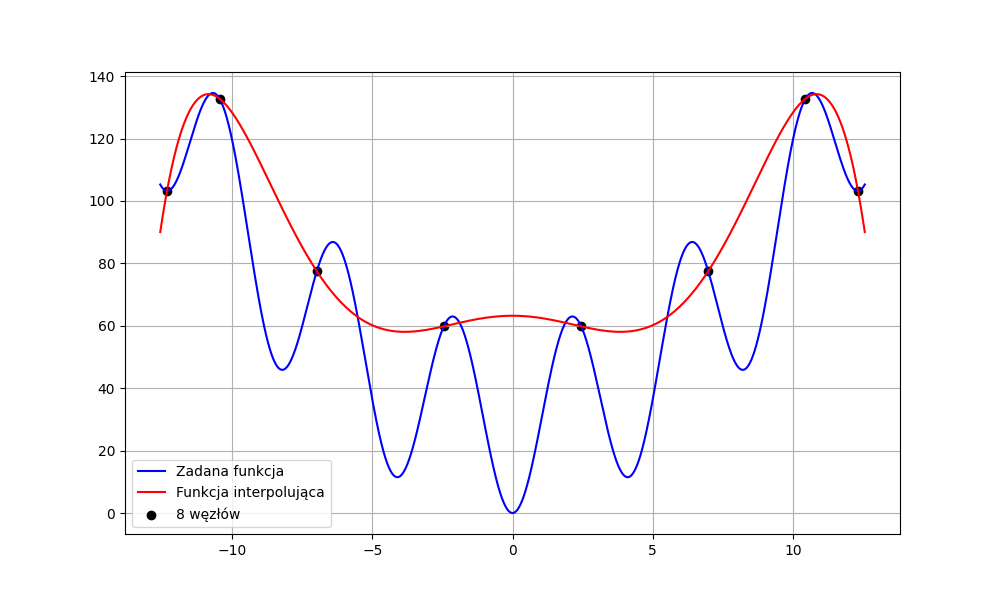
\includegraphics[width=\textwidth]{img06_n=8.png}
    \caption{Wykres dla 8 węzłów Czebyszewa}
  \end{minipage}
\end{figure}

Ponownie, przy zwiększeniu liczby węzłów Czebyszewa na krańcach przedziałów otrzymujemy dobre przybliżenie, a w środku z uwagi na mniejszą ich "gęstość" przybliżenie zaczyna się psuć, właśnie z uwagi na szybkie zmiany wartości, jak widać na poniższym wykresie.

\begin{figure}[H]
\centering
  \begin{minipage}[b]{0.49\textwidth}
    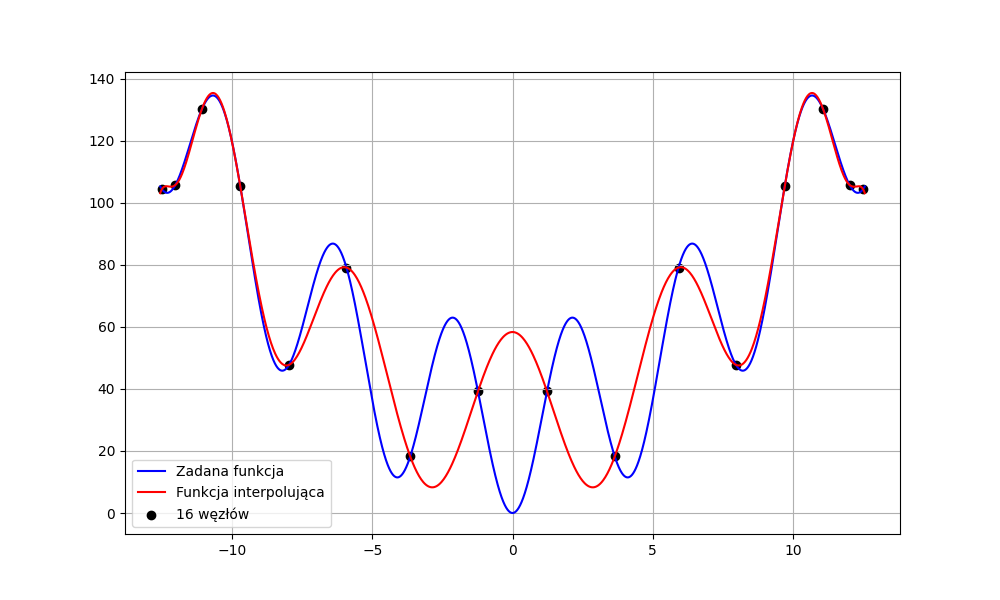
\includegraphics[width=\textwidth]{img06_n=16.png}
    \caption{Wykres dla 16 węzłów Czebyszewa}
  \end{minipage}
\end{figure}

\newpage

Zauważalny jest również problem ze zmianą wartości funkcji na krańcach przedziałów, co powoduje problemy z dopasowaniem się interpolacji w tych obszarach. Co zostało zaprezentowane na wykresie poniżej.

\begin{figure}[H]
\centering
  \begin{minipage}[b]{0.49\textwidth}
    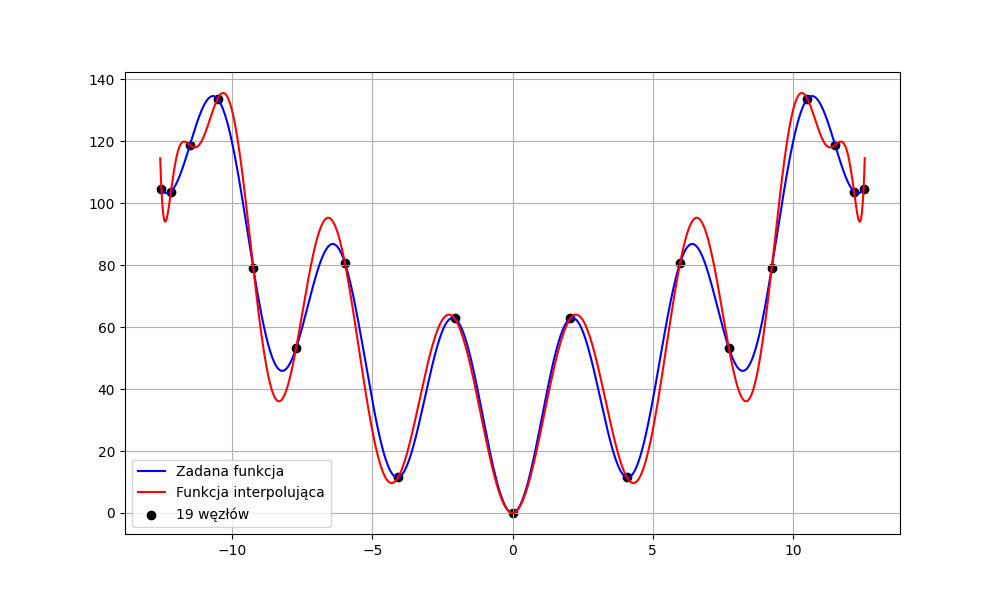
\includegraphics[width=\textwidth]{img06_n=19.png}
    \caption{Wykres dla 16 węzłów Czebyszewa}
  \end{minipage}
\end{figure}

\subsubsection{Najlepsze otrzymane przybliżenie}

Najlepsze przybliżenie ze względu na błąd maksymalny otrzymałem dla 100 węzłów czebyszewa, a ze wezględu na błąd średniokwadratowy dla 100 równoodległych węzłów. Zachodzi znaczna różnica w najlepszym przybliżeniu dla błędu maksymalnego, węzły Czebyszewa dają przybliżenie lepsze, aż o 5 rzędów wartości.

\begin{figure}[H]
  \begin{minipage}[b]{0.49\textwidth}
    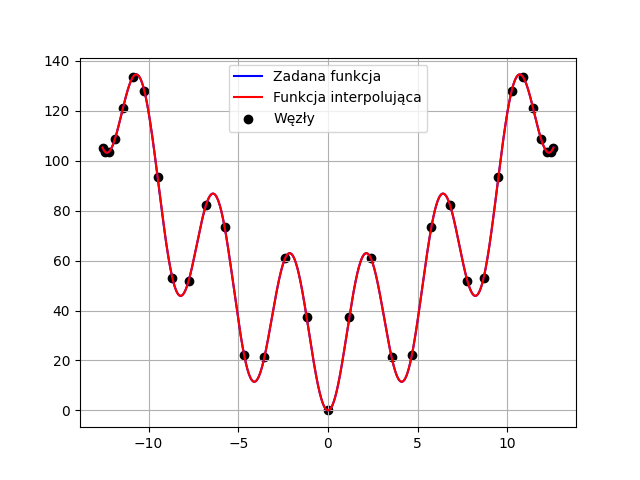
\includegraphics[width=\textwidth]{img12.png}
    \caption{Najlepsze przybliżenie ze względu na błąd maksymalny}
  \end{minipage}
  \hfill
  \begin{minipage}[b]{0.49\textwidth}
    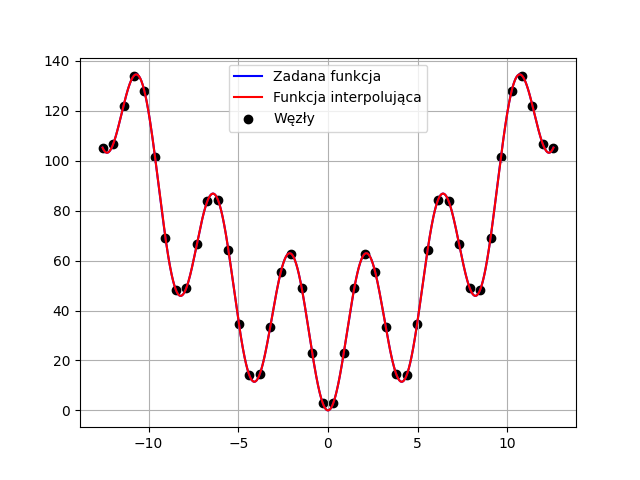
\includegraphics[width=\textwidth]{img11.png}
    \caption{Najlepsze przybliżenie ze względu na błąd średniokwadratowy}
  \end{minipage}
\end{figure}

W poniższej tabeli przedstawione są wartości błędów dla poprzednich wykresów.

\begin{table}[!ht]
    \centering
    \begin{tabular}{|l|l|}
    \hline
        Błąd maksymalny & 6.877908359115281e-05 \\ \hline
        Błąd średniokwadratowy & 8.220356191804188e-11 \\ \hline
    \end{tabular}
    \caption{Wartości błędów}
\end{table}

\newpage

\subsection{Interpolacja Hermite'a}

\subsubsection{Opis teoretyczny}

\[\mathrm{H}_{n}^{}(x) = \sum_{i = 0}^{n}\mathrm{b}_{l}^{}\mathrm{p}_{l}^{}(x) = 
\sum_{i = 0}^{k}\sum_{j=0}^{\mathrm{m}_{i}^{} - 1}\mathrm{b}_{(s(i) + j)}^{} \cdot 
\mathrm{p}_{s(i) + j}^{}(x) \]

\noindent
gdzie:

\bigbreak

\(\mathrm{p}_{s(0)}^{}(x) = 1\) 

\indent

\(\mathrm{p}_{s(i) + j}^{}(x) = \mathrm{(\mathrm{x - \mathrm{x}_{0}^{}}_{}^{})}_{}^{\mathrm{m}_{0}^{}}
\mathrm{(\mathrm{x - \mathrm{x}_{1}^{}}_{}^{})}_{}^{\mathrm{m}_{1}^{}}...
\mathrm{(\mathrm{x - \mathrm{x}_{i - 1}^{}}_{}^{})}_{}^{\mathrm{m}_{i-1}^{}}
\mathrm{(\mathrm{x - \mathrm{x}_{i}^{}}_{}^{})}_{}^{\mathrm{j}_{}^{}}\)

\indent

\(
s(i) = 
\begin{cases}
    0 & \text{dla } i = 0 \\
    \mathrm{m}_{0}^{} + \mathrm{m}_{1}^{} + ... + \mathrm{m}_{i - 1}^{} & \text{dla } i > 0
\end{cases}
\)

\indent

\(i = 0, 1, ..., k\)

\indent

\(j = 0,1,...,\mathrm{m}_{i}^{} - 1\)

\indent

Współczynniki \(\mathrm{b}_{l}^{}\) to kolejne ilorazy różnicowe.

\subsubsection{Napotkane trudności}

Podobnie jak dla interpolacji Newtona i Lagrange'a dla dość małej ilości węzłów oscylacja funkcji powoduje duży błąd w przybliżeniu, jak widać na poniższych wykresach. Dodatkowo dla węzłów równoodległych zachodzi efekt Rungego.

\begin{figure}[H]
  \begin{minipage}[b]{0.49\textwidth}
    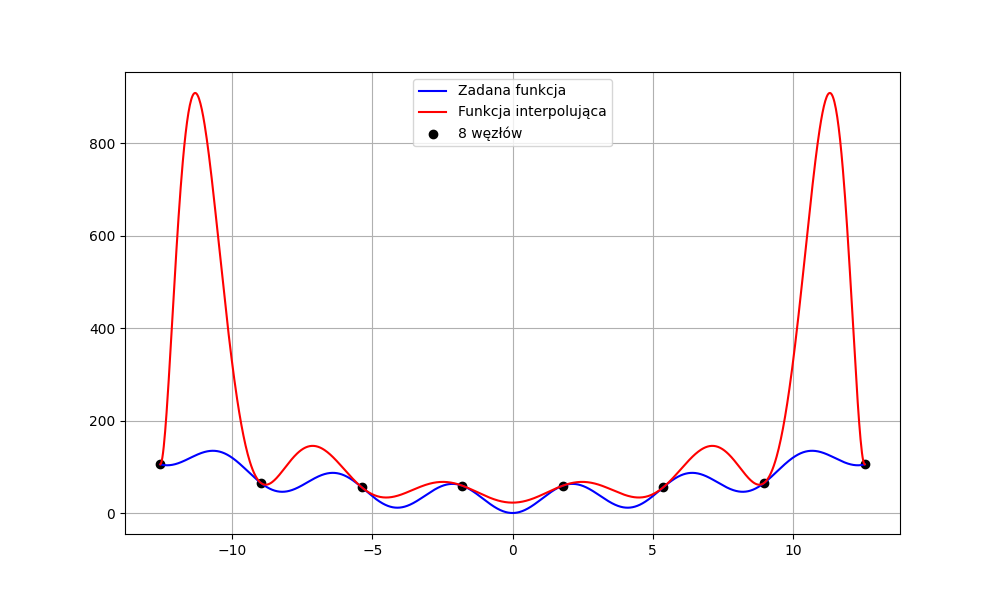
\includegraphics[width=\textwidth]{img14_n=8.png}
    \caption{Wykres dla 8 równoodległych węzłów}
  \end{minipage}
  \hfill
  \begin{minipage}[b]{0.49\textwidth}
    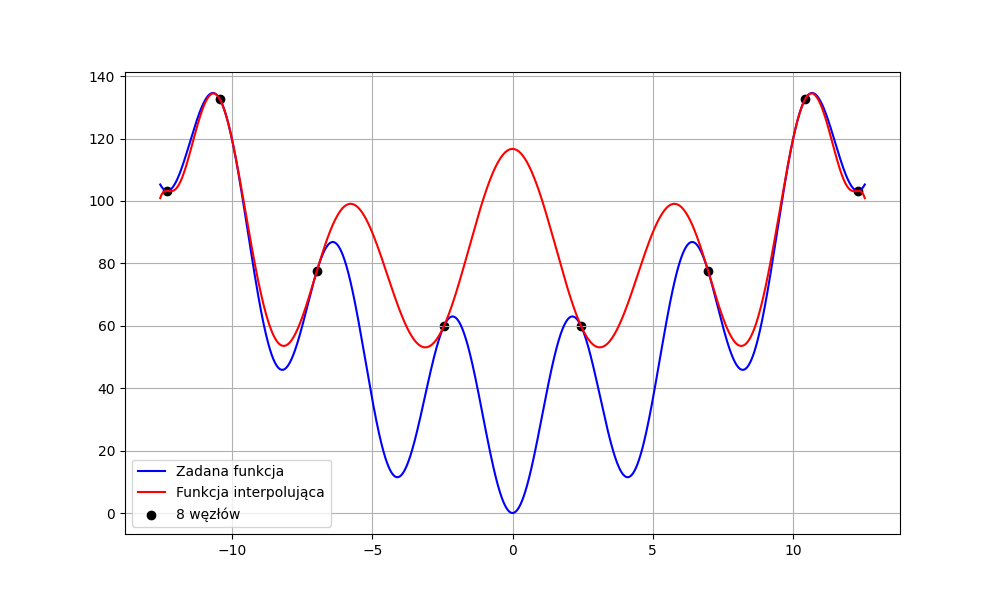
\includegraphics[width=\textwidth]{img15_n=8.png}
    \caption{Wykres dla 8 węzłów Czebyszewa}
  \end{minipage}
\end{figure}

Zupełnie przeciwnie do interpolacji Lagrange'a i Newtona dla 16 węzłów Czebyszewa otrzymujemy całkiem dobre przybliżenie. W praktyce już od 13 węzła przybliżenie jest akceptowalne, co zostało zaprezentowane poniżej.

\begin{figure}[H]
\centering
  \begin{minipage}[b]{0.49\textwidth}
    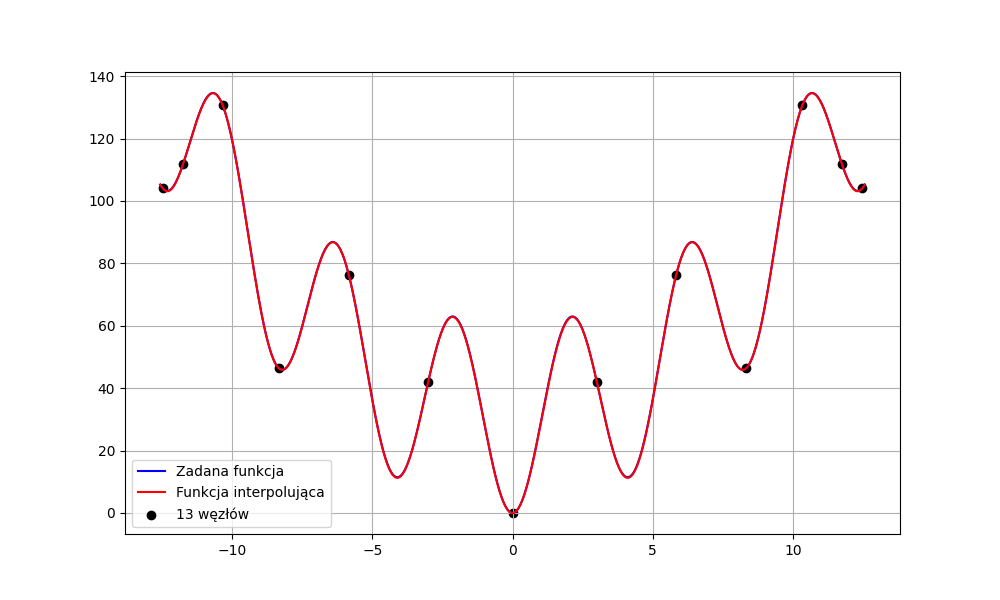
\includegraphics[width=\textwidth]{img15_n=13.png}
    \caption{Wykres dla 13 węzłów Czebyszewa}
  \end{minipage}
\end{figure}

Jeśli chodzi o problem z znaczym wzrostem wartości funkcji, to praktycznie tutaj nie występuje. Prawdopodobnie dzieje się tak ze względu na wykorzystanie pochodnej funkcji do obliczeń.

Dodatkowym problemem w interpolacji Hermite'a był znaczny błąd przybliżenia występujący na krawędzi przedziału, który zwiększał się wraz z wzrostem liczby węzłów. Ta sytuacja została pokazana na wykresie poniżej.

\begin{figure}[H]
\centering
  \begin{minipage}[b]{0.49\textwidth}
    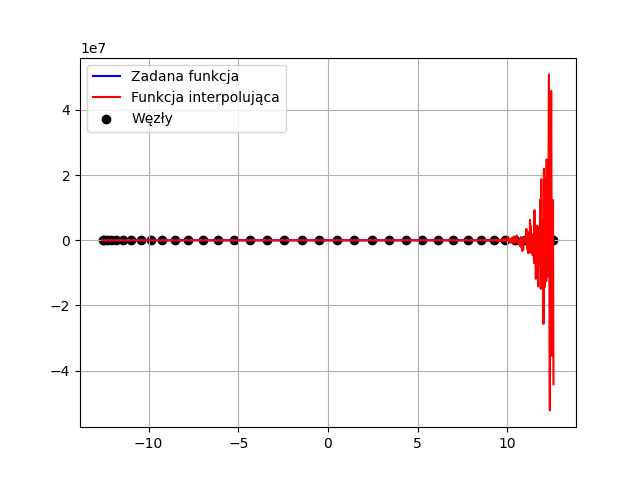
\includegraphics[width=\textwidth]{img18.png}
    \caption{Wykres dla 40 węzłów Czebyszewa}
  \end{minipage}
\end{figure}

\subsubsection{Najlepsze otrzymane przybliżenie}

Jak widać dla najmniejszego błędu maksymalneggo dostajemy dobre przybliżenie, ale ze względu na błąd średniokwadratowy wcale tak nie jest, a błąd przybliżenia na krańcu przedziału jest bardzo duży.

\begin{figure}[H]
  \begin{minipage}[b]{0.49\textwidth}
    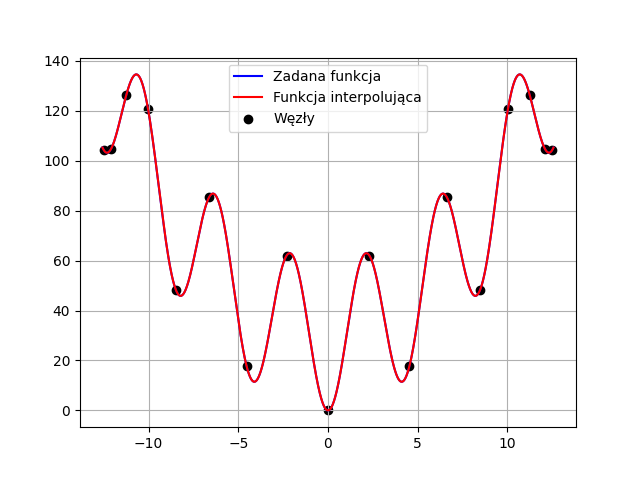
\includegraphics[width=\textwidth]{img16.png}
    \caption{Najlepsze przybliżenie ze względu na błąd maksymalny}
  \end{minipage}
  \hfill
  \begin{minipage}[b]{0.49\textwidth}
    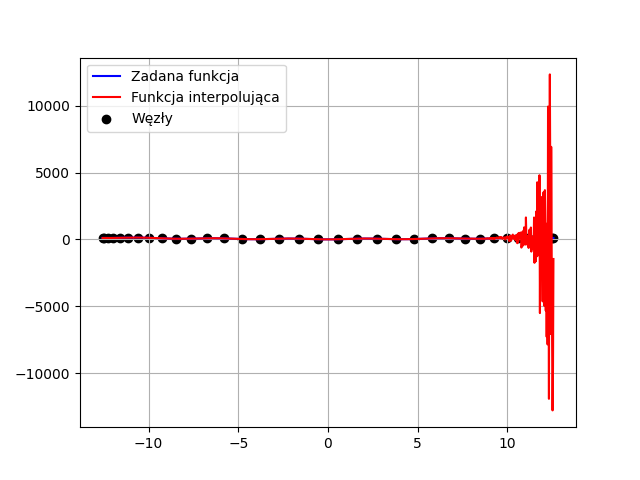
\includegraphics[width=\textwidth]{img17.png}
    \caption{Najlepsze przybliżenie ze względu na błąd średniokwadratowy}
  \end{minipage}
\end{figure}

W tabeli poniżej przedstawione zostały wartości błędów dla powyższych wykresów

\begin{table}[!ht]
    \centering
    \begin{tabular}{|l|l|}
    \hline
        Błąd maksymalny & 0.0002819640489661879 \\ \hline
        Błąd średniokwadratowy & 5.6728812264079556e-11 \\ \hline
    \end{tabular}
    \caption{Wartości błędów}
\end{table}

\newpage

\subsection{Interpolacja funkcją sklejaną 2-go stopnia}

\subsubsection{Opis teoretyczny}

\paragraph{Wyznaczanie współczynników}
\bigbreak

Kwadratowa funkcja sklejona musi spełniać warunki:

\begin{itemize}
    \item \( S_i (x) = a_i + b_i(x - x_i) + c_i(x - x_i)^2\) \ (1)
    \item \(S_i(x_i) = f(x_i) = y_i\) (2)
    \item \(s_i(\mathrm{x}_{i+1}^{}) = S_{i + 1}(x_{i+1})\) \ (3)
    \item \(S'_i(x_{i+1}) = S'_{i+1}(x_{i+1})\) \ (4)
\end{itemize}

\noindent
Podstawiam \(x_i\) do (1) i korzystam z właności (2), z tego otrzymuję:

\[y_i = S_i (x_i) = a_i + b_i(x_i - x_i) + c_i(x_i - x_i)^2 = a_i \Rightarrow  a_i = y_i \ \ (5)\] 
\noindent
Korzystając z warunku (1) i (4):

\[b_{i+1} + 2c_{i+1}(x_{i+1}-x_{i+1}) = b_i + 2c_i(x_{i+1} - x_i)\]

\[b_{i+1} = b_i + 2c_i(x_{i+1} - x_i)\]

\[c_i = \frac{b_{i+1}-b_i}{2(x_{i+1}-x_i)} \ \ (6)\] 
\noindent
Korzystając z (1), (2), (3) i (5):

\[y_{i+1} = S_i(x_{i+1}) = S_{i+1}(x_{i+1}) = y_i + b_i(x_{i+1} - x_i) + c_i(x_{i+1}-x_i)^2 \ \ (7)\]
\noindent
Korzystając z (6) i (7):

\[y_{i+1} - y_i = b_i(x_{i+1}-x_i) + \frac{b_{i+1}-b_i}{2(x_{i+1}-x_i)}(x_{i+1}-x_i)^2\]

\[\frac{y_{i+1} - y_i}{x_{i+1}-x_i} = b_i + \frac{1}{2}b_{i+1} - \frac{1}{2}b_i\]

\[2\cdot \frac{y_{i+1} - y_i}{x_{i+1}-x_i} = b_{i+1}+b_i\]

\[b_i + b_{i-1} = 2\frac{y_i - y_{i-1}}{x_i - x_{i-1}}\]
\noindent
Oznaczam \(\frac{y_i - y_{i-1}}{x_i - x_{i-1}}\) jako \(v\) i tworzę układ równań w celu wyliczenia
wspołczynnika \(b_i\)

\bigbreak

\[b_1 + b_2 = 2v_2\]
\[b_2 + b_3 = 2v_3\]
\[\vdots\]
\[b_{n-2}+b_{n-1}=2v_{n-1}\]

\begin{gather*}
\begin{bmatrix}
1 & 1 & 0 & \cdots & 0 \\
0 & 1 & 1 & \ddots & \vdots \\
\vdots & \ddots & \ddots & \ddots & 0 \\
0 & \cdots & 0 & 1 & 1 
\end{bmatrix}  
\begin{bmatrix}
b_1 \\
b_2 \\
\vdots \\
b_{n-1} 
\end{bmatrix} 
=
\begin{bmatrix}
2v_1 \\
2v_2 \\
\vdots \\
2v_{n-1} 
\end{bmatrix}
\end{gather*}
\noindent
Jak widać jest n - 1 równań i n niewiadowmych, zatem trzeba będzie ustalić doddatkowy warunek brzegowy.

\paragraph{Natural Boundary}

Założenia:

\[S'_1(x_1) = 0 \ \ \vee \ \ S'_{n-1}(x_n) = 0 \ \ (8)\]
\noindent
Korzystając z (1) i (8):

\[S'_1(x_1) = 0 = b_1 + 2c_1(x_1-x_1) \Rightarrow b_1 = 0 \ \ (9)\]
\noindent
Zatem:

\[b_1+b_2 = 2v_2 \Rightarrow b_2 = 2v_2\]

\[b_2 + b_3 = 2v_3 \Rightarrow b_3 = 2v_3-2v_2\]

\[\vdots\]

\[b_n = 2(v_n-v_{n-1}+v_{n-2}-...\pm v_2)\]

\paragraph{Clamped Boundary}
\noindent
Założenia:

\[S'_1(x_1) = f'_1(x) \ \ \vee \ \ S'_{n-1}(x_n) = f'_{n-1}(x) \ \ (10)\]
\noindent
\(f'_1(x)\) można zapisać jako:
\[f'_1(x) = \frac{y_2-y_1}{x_2-x_1} \ \ (11)\]
\noindent
Korzystając z (1), (10) i (11):

\[b_1 + 2c_1(x_1 - x_1) = \frac{y_2 - y_1}{x_2-x_1} \Rightarrow  b_1 = \frac{y_2 - y_1}{x_2-x_1} = v_2\]

\bigbreak
\noindent
Zatem:

\[b_1 + b_2 = 2v_2 \Rightarrow b_2 = v_2\]

\[b_2 + b_3 = 2v_3 \Rightarrow b_3 = 2v_3 - v_2 \]

\[\vdots \]

\[b_n = 2(v_n-v_{n-1}+v_{n-2}+...\pm v_3) \pm v_2\]

\newpage

\subsection{Napotkane trudności}

Ponownie dla małej liczby węzłów przybliżenie nie było najlepsze ze względu na duże oscylacje funkcji, jak widać na poniższych wykresach.

\begin{figure}[H]
  \begin{minipage}[b]{0.49\textwidth}
    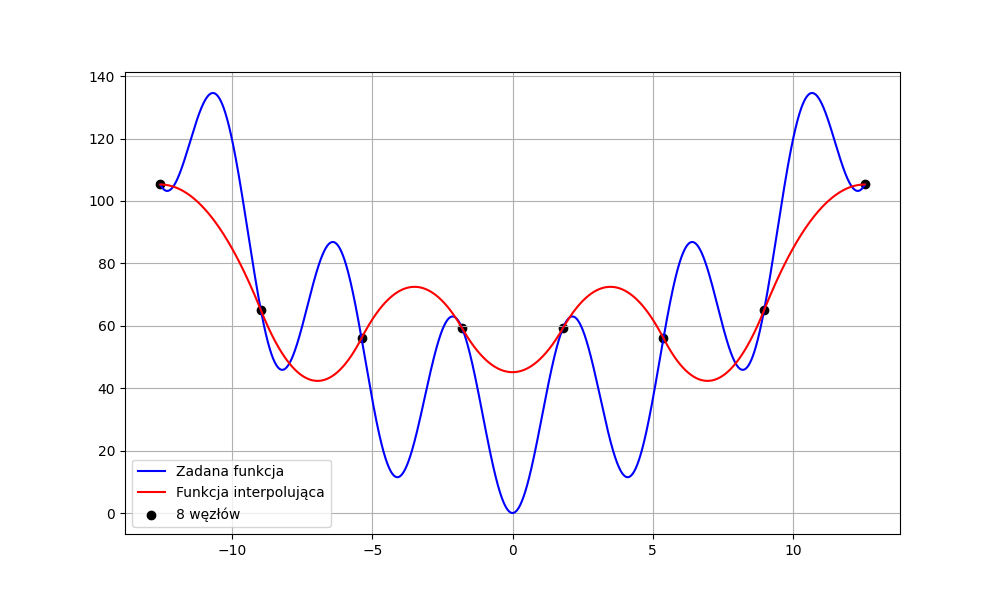
\includegraphics[width=\textwidth]{img19_n=8.png}
    \caption{Wykres dla 8 równoodległych węzłów i Natual Boundary}
  \end{minipage}
  \hfill
  \begin{minipage}[b]{0.49\textwidth}
    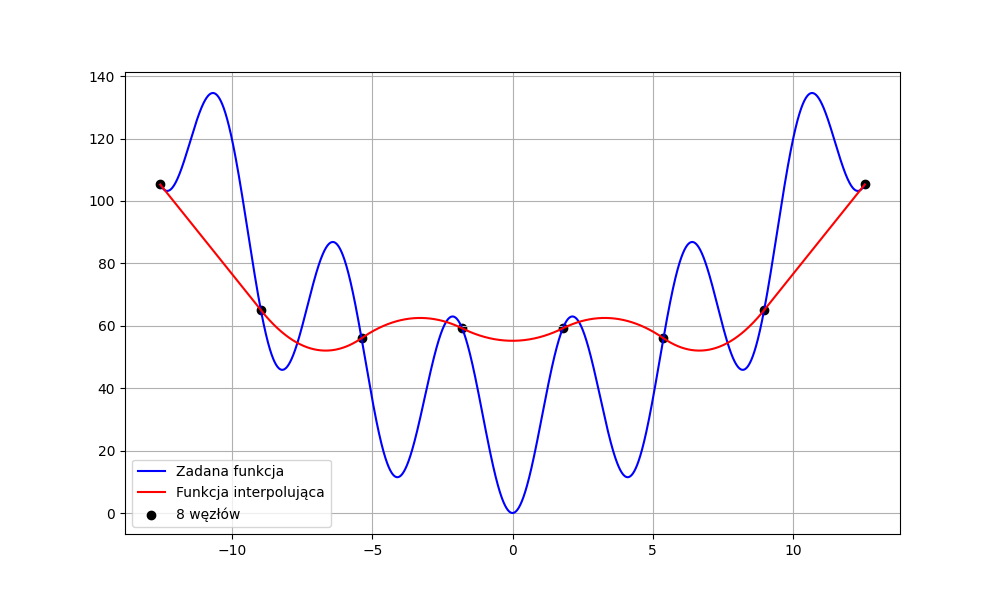
\includegraphics[width=\textwidth]{img20_n=8.png}
    \caption{Wykres dla 8 równoodległych węzłów i Clamped Boundary}
  \end{minipage}
\end{figure}

Przy wykorzystaniu funkcji sklejanej 2-go stopnia występowały problemy z dopasowaniem funkcji interpolującej w punktach przegięcia funkcji, co zostało zaprezentowane poniżej. Problem ten występował zarówno dla Natural Boundary, jak i clamped Boundary. Na szczęscie wzraz z zwiększeniem liczby węzłów problem znika.

\begin{figure}[H]
  \begin{minipage}[b]{0.49\textwidth}
    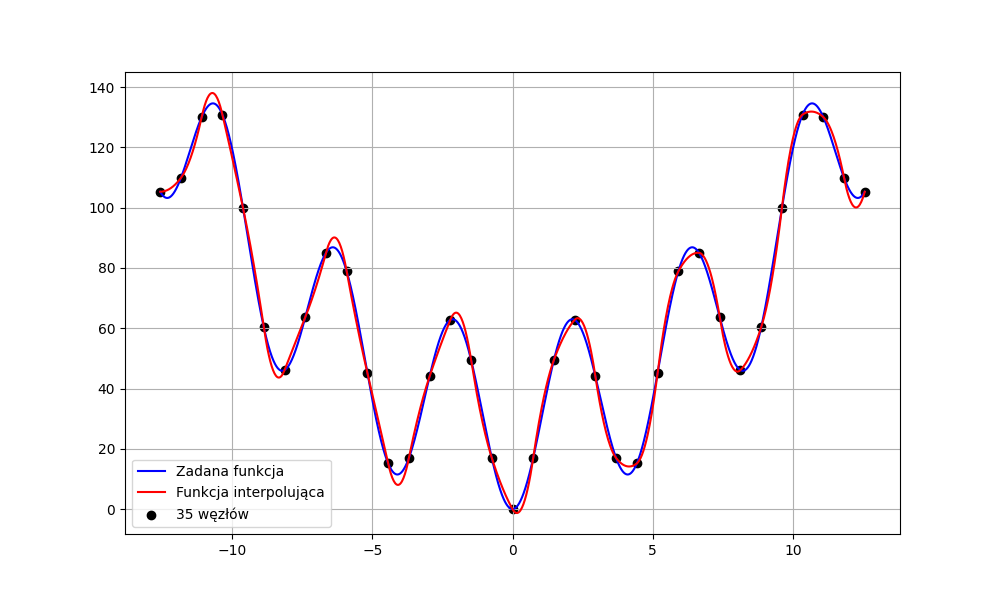
\includegraphics[width=\textwidth]{img19_n=35.png}
    \caption{Wykres dla 35 równoodległych węzłów i Natual Boundary}
  \end{minipage}
  \hfill
  \begin{minipage}[b]{0.49\textwidth}
    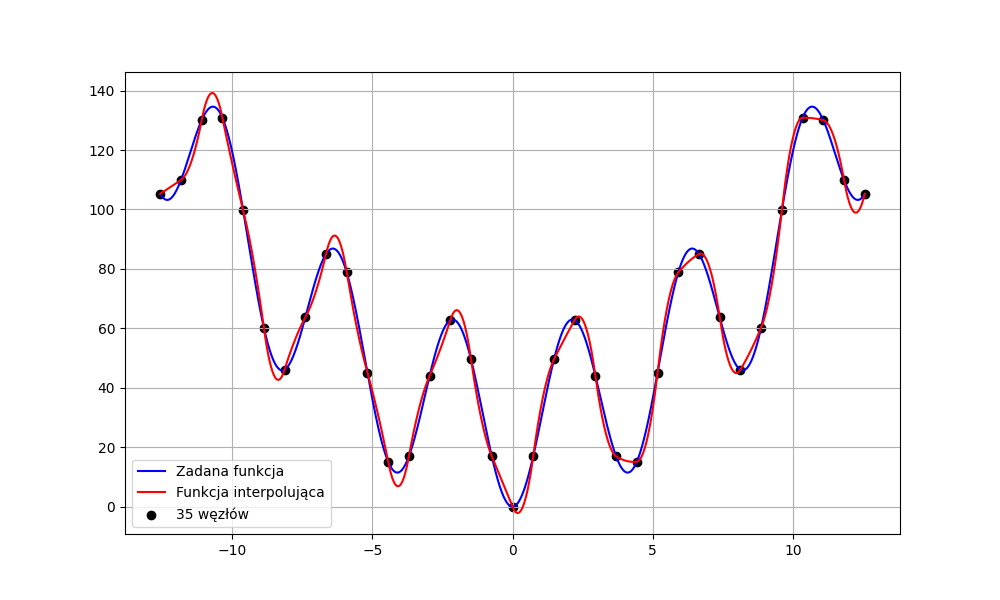
\includegraphics[width=\textwidth]{img20_n=35.png}
    \caption{Wykres dla 35 równoodległych węzłów i Clamped Boundary}
  \end{minipage}
\end{figure}

\newpage

Występowały też dosć osobliwe błędy w losowych miejscach. Jak widać poniżej funkcja jest dopasowana dość dobrze w większości miejsc, jednak w paru występuje znaczny błąd. Taka sama własność zachodzi dla Natural Boundary i Clamped Boundary, a miejsca, w których zachodzą błędy zmieniają się wraz z zmianą liczby węzłów.

\begin{figure}[H]
\centering
  \begin{minipage}[b]{0.49\textwidth}
    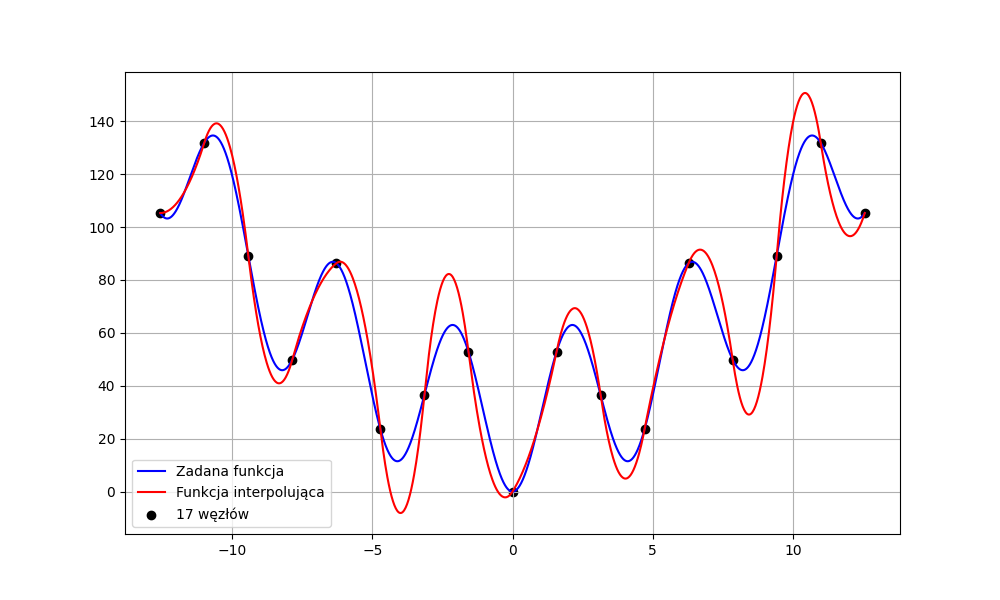
\includegraphics[width=\textwidth]{img19_n=17.png}
    \caption{Wykres dla 17 równoodległych węzłów i Natural Boundary}
  \end{minipage}
\end{figure}


\subsubsection{Najlepsze otrzymane przybliżenie}

W przypadku funkcji sklejanej 2-go stopnia przybliżenie polepsza się wraz z zwiększeniem liczby węzłów, zatem najlepsze przybliżenie w obu przypadkach otrzymałem dla 100 węzłów. Jak widać jest to dobre przybliżenie

\begin{figure}[H]
\centering
  \begin{minipage}[b]{0.49\textwidth}
    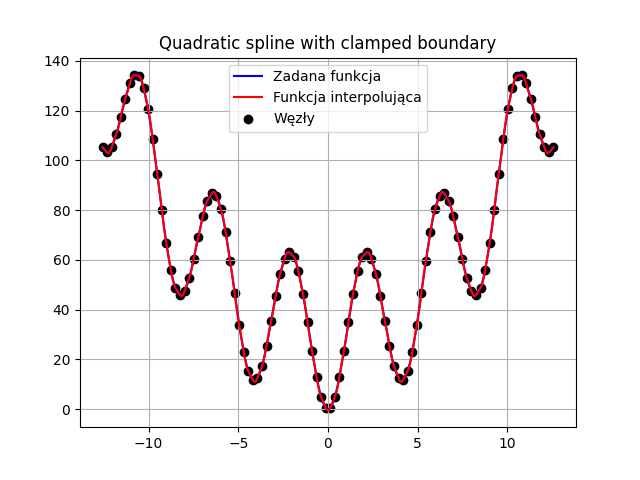
\includegraphics[width=\textwidth]{img21.png}
    \caption{Najlepsze przybliżenie funkcji ze względu na błąd maksymalny i średniokwadratowy}
  \end{minipage}
\end{figure}

W tabeli poniżej przedstawiono wartości błędów dla powyższych wykresów.

\begin{table}[!ht]
    \centering
    \begin{tabular}{|l|l|}
    \hline
        Błąd maksymalny & 0.5527769402251668 \\ \hline
        Błąd średniokwadratowy & 0.16001239042418153 \\ \hline
    \end{tabular}
    \caption{Wartości błędów}
\end{table}

\newpage

\subsection{Funkcja sklejana 3-go stopnia}

\paragraph{Wyznaczanie współczynników}

Wzór na sześcienną funkcję sklejaną został podany poniżej:

\[s(x) = \mathrm{a}_{i}^{} + \mathrm{b}_{i}^{}\cdot (x - \mathrm{x}_{i}^{}) +\mathrm{c}_{i}^{}\cdot \mathrm{(x - \mathrm{x}_{i}^{})}_{}^{2} + \mathrm{d}_{i}^{}\cdot  \mathrm{(x-\mathrm{x}_{i}^{})}_{}^{3} \ dla \ x \in [\mathrm{x}_{i}^{}, \mathrm{x}_{i + 1}^{}]\]
\noindent
Dodatkowo funkcja sklejana 3-go stopnia musi spełniać poniższe warunki:
\begin{itemize}
\item \(S_i(x_{i+1}) = f(x_{i+1})\)
\item \(S_i(x_{i+1}) = S_{i+1}(x_{i+1})\)
\item \(S'i(x_{i+1}) = S'_{i+1}(x_{i+1})\)
\item \(S''(x_{i+1}) = S''_{i+1}(x_{i+1})\)
\end{itemize}
\noindent
Ponieważ \(S_i(x)\) jest sześcienna, to \(S''_i(x)\) jest liniowa na przedziale \([x_i, x_{i+1}]\). Wprowadzam \(h_i = x_{i+1} - x_i\), wtedy:

\[S''_i(x) = S''_i(x_i)\frac{x_{i+1}-x}{h_i} + s''_i(x_{i+1})\frac{x-x_i}{h_i}\]
\noindent
Całkując dwukrotnie otrzymuję:

\[S_i(x) = \frac{S''_i(x_i)}{6h_i}(x_{i+1}-x)^3 + \frac{S''_i(x_{i+1})}{6h_i}(x-x_i)^3+C(x-x_i)+D(x_{i+1}-x)\],
\noindent
gdzie C i D - stałe całkowania
\noindent
Korzystając z warunków interpolacji:
\noindent
\(S_i(x_i) = y_i\) oraz \(S_i(x_{i+1}) = y_{i+1}\) można wyliczyć C i D. Po wyliczeniu tych stałych otrzymujemy:

\[S_i(x) = \frac{S''_i(x_i)}{6h_i}(x_{i+1}-x)^3 + \frac{S''_i(x_{i+1})}{6h_i}(x-x_i)^3 + 
(\frac{y_{i+1}}{h_i} - \frac{S''_i(x_{i+1})h_i}{6})(x-x_i) + (\frac{y_i}{h_i}-\frac{S''_i(x_i)h_i}{6})(x_{i+1}-x)\]
\noindent
W powyższym wzorze nadal nie znamy \(S''_i(x)\). W celu jego wyliczenia należy skorzystać z warunku ciągłości pierwszech pochodnej. Różniczkuję zatem \(S_i(x)\):

\[S'_i(x_i) = -\frac{h_i}{3}S''_i(x_i) - \frac{h_i}{6}S''_i(x_{i+1}) - \frac{y_i}{h_i} + \frac{y_{i+1}}{h_i}\]
\noindent
Dla przejrzystości należy wprowadzić dwa symbole:
\begin{itemize}
\item \(\sigma_i = \frac{1}{6}S''(x_i)\)
\item \(\Delta_i = \frac{y_{i+1}-y_i}{h_i}\)
\end{itemize}
\noindent
Wtedy:

\[S'_i(x_i) = -2\sigma_ih_i - \sigma_{i+1}h_i + \Delta_i\]
\[S'_i(x_i) = \Delta_i - h_i(\sigma_{i+1}+2\sigma_i)\]
\noindent
Wtedy:

\[S'_{i-1}(x_i) = \Delta_{i-1} + h_{i-1}(2\sigma_i + \sigma_{i-1})\]
\noindent
Teraz korzystając z warunku ciągłości (\(S'_{i-1}(x_i) = S'_i(x_i)\)):

\[\Delta_{i-1} + h_{i-1}(2\sigma_i + \sigma_{i-1}) = \Delta_i - h_i(\sigma_{i+1} + 2\sigma_i)\]
\noindent
Finalnie otrzymujemy układ równań liniowych:

\[h_{i-1}\sigma_{i-1} + 2(h_{i-1}+h_i)\sigma_i + h_i\sigma_{i+1} = \Delta_i - \Delta_{i-1}, i = 2,3,...,n-1\]
\noindent
Jak można zauważyć w układzie równań mamy n niewiadomych i n - 2 równań, zatem należy określić dwa dodatkowe warunki brzegowe.

\paragraph{Default Boundary}

Warunki:

\begin{itemize}
\item \(C_1(x)\) - f. sześcienna przez pierwsze 4 punkty
\item \(C_n(x)\) - f. sześcienna przez ostatnie 4 punkty
\end{itemize}

\[S'''(x_1) = C'''_1 \ \ \ S'''(x_n) = C'''_n\]
\noindent
Stałe \(C'''_1 i C'''_n\) mogą być określone bez znajomości \(C_1(x)\) i \(C_n(x)\):

\begin{itemize}
\item \(\Delta_i^{(1)} = \frac{y_{i+1} - y_i}{x_{i+1}-x_i}\)
\item \(\Delta_i^{(2)} = \frac{\Delta_{i+1}^{(1)}-\Delta_i^{(1)}}{x_{i+2}-x_i}\)
\item \(\Delta_i^{(3)} = \frac{\Delta_{i+1}^{(2)}-\Delta_i^{(2)}}{x_{i+3}-x_i}\)
\end{itemize}
\noindent
Różniczkując wzór na \(S''(x)\) na przedziale \([x_i, x_{i+1}]\), otrzymujemy:

\[S'''(x_1) = C'''_1(x_1) \Rightarrow  \frac{6}{h_1}(\sigma_2-\sigma_1) = 6\Delta_i^{(3)}\]

\[S'''(x_n) = C'''_n(x_n) \Rightarrow  \frac{6}{h_{n-1}}(\sigma_n - \sigma_{n-1}) = 6\Delta_{n-3}^{(3)}\]
\noindent
Po przekształceniu otrzymujemy:

\begin{itemize}
\item \(-h_1\sigma_1 + h_1\sigma_2 = h_1^2\Delta_1^{(3)}\)
\item \(h_{n-1}\sigma_{n-1} - h_{n-1}\sigma_n = -h_{n-1}^2\Delta_{n-3}^{(3)}\)
\end{itemize}
\noindent
Finalnie otrzymujemy:

\begin{gather*}
\begin{bmatrix}
-h_1 & h_1 & 0 & 0 & 0 \\
h_1 & 2(h_1+h_2) & h_2 & 0 & 0 \\
0 & h_2 & 2(h_2+h_3) & h_3 & 0 \\
\vdots & \vdots & \vdots & \vdots & \vdots \\
0 & 0 & h_{n-2} & 2(h_{n-2} + h_{n-1}) & h_{n-1} \\
0 & 0 & 0 & h_{n-1} & -h_{n-1} 
\end{bmatrix}
\begin{bmatrix}
\sigma_1 \\
\sigma_2 \\
\sigma_3 \\
\vdots \\
\sigma_{n-1} \\
\sigma_n 
\end{bmatrix}
=
\begin{bmatrix}
\mathrm{h}_{1}^{2}\mathrm{\Delta}_{1}^{(3)} \\
\Delta_2 - \Delta_1 \\
\Delta_3 - \Delta_2 \\
\vdots \\
\mathrm{\Delta}_{n-1}^{} - \mathrm{\Delta}_{n-2}^{} \\
\mathrm{-h}_{n-1}^{2}\mathrm{\Delta}_{n-3}^{(3)} 
\end{bmatrix}
\end{gather*}

\paragraph{Natural Boundary}

Warunki:

\[S''(x_1) = S''(x_n) = 0\]
\noindent
Biorąc pod uwagę, że \(\sigma_i = \frac{1}{6}S''_i(x_i)\) otrzymujemy:

\[S''(x_1) = S''_1(x_1) = 0 \Leftrightarrow \sigma_1 = 0\]

\[S''(x_n) = S''_n(x_n) = 0 \Leftrightarrow \sigma_n = 0\]
\noindent
Dzięki temu otrzymujemy:

\begin{gather*}
\begin{bmatrix}
1 & 0 & 0 & 0 & 0 \\
h_1 & 2(h_1+h_2) & h_2 & 0 & 0 \\
0 & h_2 & 2(h_2+h_3) & h_3 & 0 \\
\vdots & \vdots & \vdots & \vdots & \vdots \\
0 & 0 & h_{n-2} & 2(h_{n-2} + h_{n-1}) & h_{n-1} \\
0 & 0 & 0 & 0 & 1 
\end{bmatrix}
\begin{bmatrix}
\sigma_1 \\
\sigma_2 \\
\sigma_3 \\
\vdots \\
\sigma_{n-1} \\
\sigma_n 
\end{bmatrix}
=
\begin{bmatrix}
0 
\Delta_2 - \Delta_1 \\
\Delta_3 - \Delta_2 \\
\vdots \\
\mathrm{\Delta}_{n-1}^{} - \mathrm{\Delta}_{n-2}^{} \\
0
\end{bmatrix}
\end{gather*}

\newpage

\subsection{Napotkane trudności}

Jak w przypadku innych metod interpolacji występuje problem z przybliżeniem z powodu dużej oscylacji wartości funkcji. Występuje on zarówno dla Default Boundary, jak i Natural Boundary.

\begin{figure}[H]
  \begin{minipage}[b]{0.49\textwidth}
    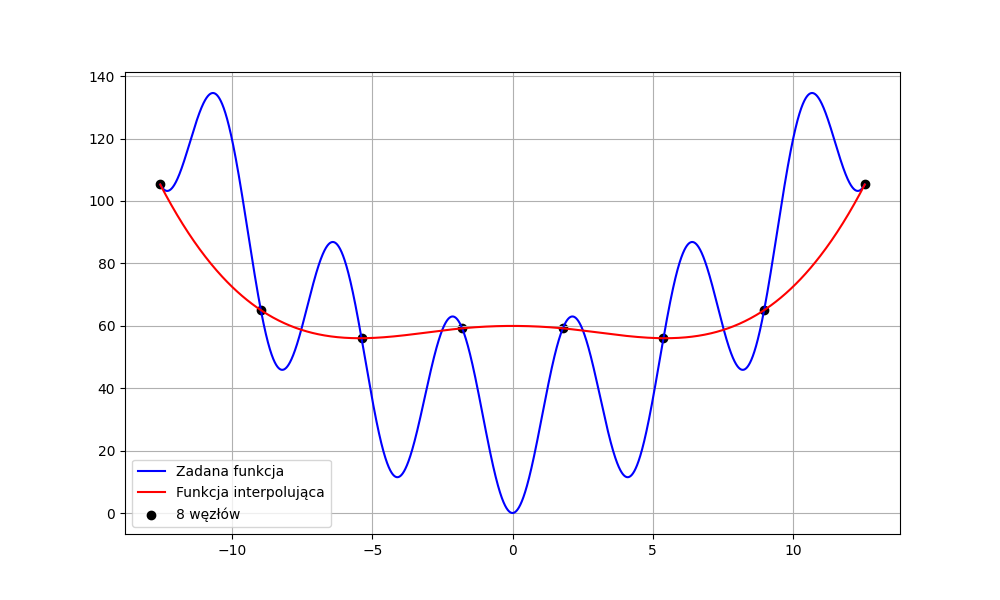
\includegraphics[width=\textwidth]{img23_n=8.png}
    \caption{Wykres dla 8 równoodległych węzłów i Default Boundary}
  \end{minipage}
  \hfill
  \begin{minipage}[b]{0.49\textwidth}
    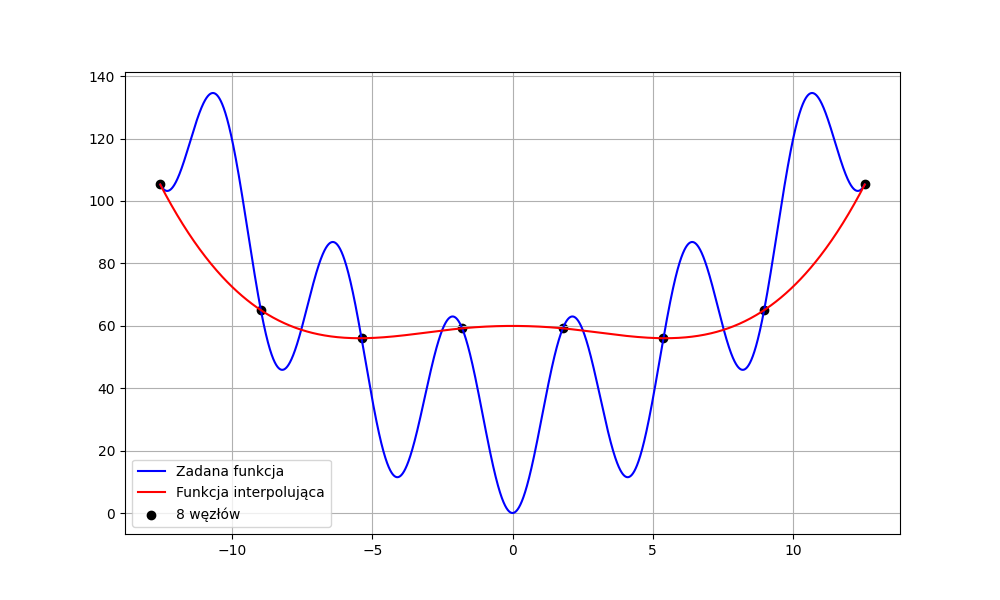
\includegraphics[width=\textwidth]{img23_n=8.png}
    \caption{Wykres dla 8 równoodległych węzłów i Natural Boundary}
  \end{minipage}
\end{figure}

Widoczny był też problem z przybliżeniem na krańcach przedziałów. Został on zaprezentowany poniżej. Błąd ten występuje zarówno dla małej, jak i dużej liczby węzłów i jest bardziej widoczny dla Natural Boundary, a dla Default Boundary znacznie szybciej zanika.

\begin{figure}[H]
  \begin{minipage}[b]{0.49\textwidth}
    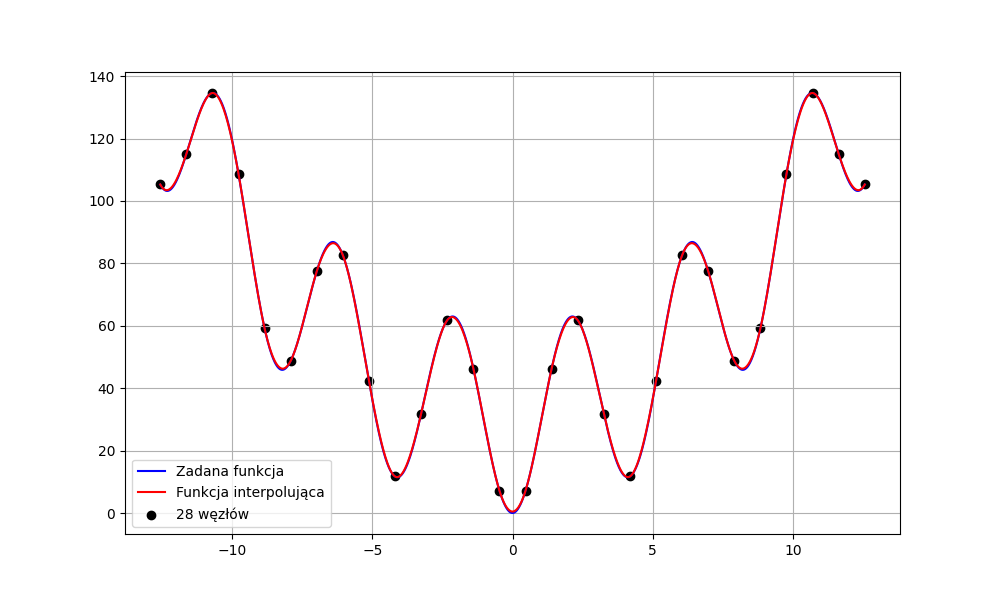
\includegraphics[width=\textwidth]{img23_n=28.png}
    \caption{Wykres dla 28 równoodległych węzłów i Default Boundary}
  \end{minipage}
  \hfill
  \begin{minipage}[b]{0.49\textwidth}
    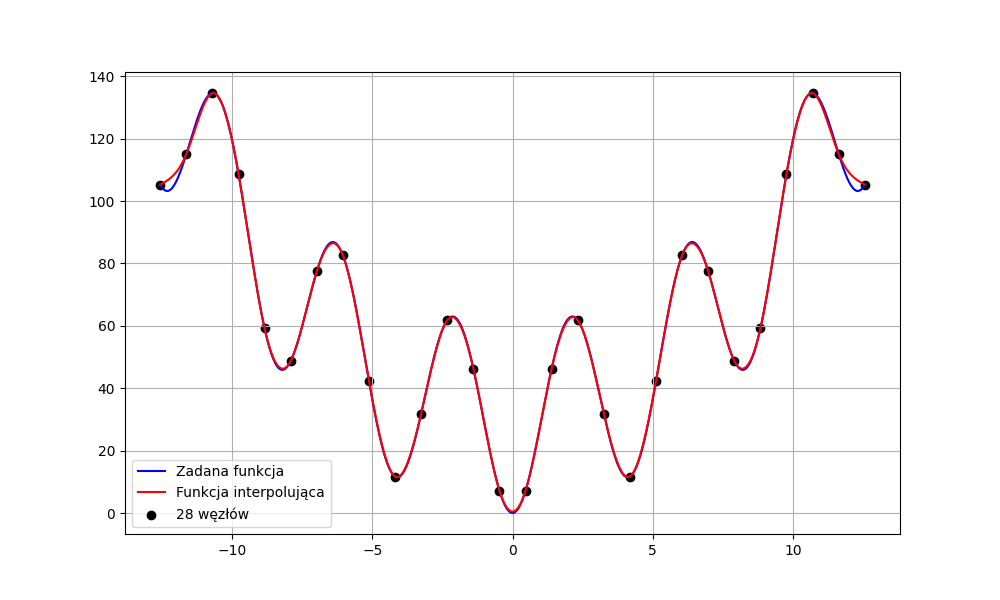
\includegraphics[width=\textwidth]{img24_n=28.png}
    \caption{Wykres dla 28 równoodległych węzłów i Natural Boundary}
  \end{minipage}
\end{figure}

Dla 13 równoodległych węzłów i Natural Boundary otrzymałem bardzo "szczęśliwe" ułożenie węzłów, które dało bardzo dobre przybliżenie w środku przedziału. Natomiast widoczny jest problem z przybliżeniem na krańcach przedziałów, ze względu na znaczny wzrost wartości funkcji w tym obszarze/

\begin{figure}[H]
\centering
  \begin{minipage}[b]{0.49\textwidth}
    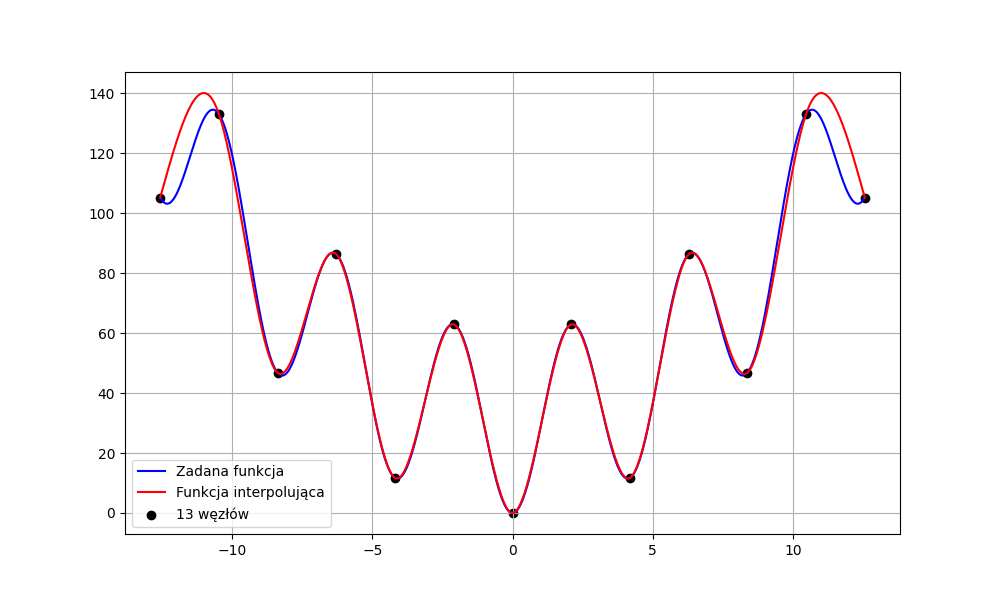
\includegraphics[width=\textwidth]{img24_n=13.png}
    \caption{Dobre przybliżenie dla 13 równoodległych węzłów i Natural Boundary}
  \end{minipage}
\end{figure}

\subsubsection{Najlepsze otrzymane przybliżenie}

Najlepsze przybliżenie zarówno ze względu na błąd maksymalny, jak i średniokwadratowy otrzymałem dla 50 równoodległych węzłów i Default Boundary. Otrzymane przybliżenie jest zadowalająće.

\begin{figure}[H]
\centering
  \begin{minipage}[b]{0.49\textwidth}
    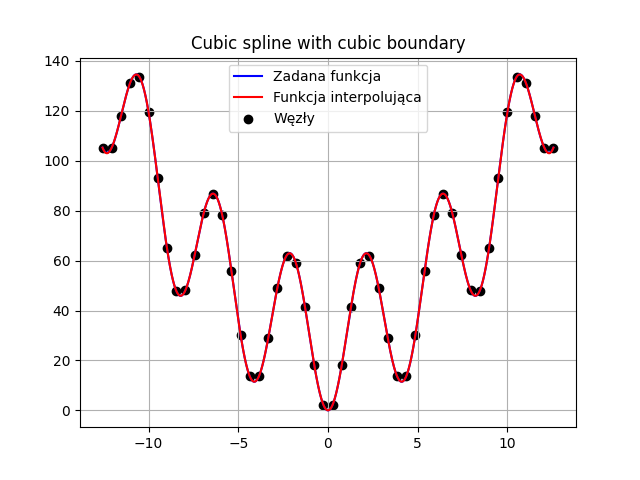
\includegraphics[width=\textwidth]{img25.png}
    \caption{Najlepsze przybliżenie ze względu na błąd maksymalny i średniokwadratowy}
  \end{minipage}
\end{figure}

Poniżej w tabeli przedstawione są wartości błędów dla powyższych wykresów

\begin{table}[!ht]
    \centering
    \begin{tabular}{|l|l|}
    \hline
        Błąd maksymalny & 0.2206113875498943 \\ \hline
        Błąd średniokwadratowy & 0.0012792870753556306 \\ \hline
    \end{tabular}
    \caption{Wartości błędó}
\end{table}

\newpage

\section{Aproksymacja średniokwadratowa wielomianami algebraicznymi}

\subsubsection{Opis teoretyczny}

\noindent
Funkcja bazowe, czyli ciągi jednomianów \(\varphi _j(x) = x^i, j = 0, 1, ..., m\)

\noindent
Funkcja aproksymująca: \(f(x) = \sum_{j=0}^{m}a_j\varphi_j(x) = \sum_{j=0}^{m}a_jx^i\)

\noindent
F(x) - zadana na zbiorze dyskretnym \(\{x_i\}, i = 0, 1, ..., n\)

\noindent
Szukamy takich współczynników \(a_j\), że:

\[min!\sum_{i=0}^{n}w(x_i)[F(x_i) - f(x_i)]^2\]

\noindent
Układ normalny:

\[\sum_{i = 0}^{n}w(x_i)[F(x_i) - \sum_{j=0}^{m}a_jx_i^j]x_i^{k\longleftarrow \frac{\partial f}{\partial a_k}} = 0, k = 0, 1, ..., m\]

\[\sum_{i = 0}^{n}w(x_i)x_i^k\sum_{j=0}^{m}a_jx_i^j = \sum_{i=0}^{n}w(x_i)F(x_i)x_i^k, k =0,1,...,m\]

\[\sum_{j=0}^{m}(\sum_{i=0}^{n}w(x_i)x_i^{j+k}a_j = \sum_{i=0}^{n}w(x_i)F(x_i)x_i^k\]

\noindent
W postaci macierzowej:

\begin{gather*}
\begin{pmatrix}
\Sigma w_i & \Sigma w_ix_i & \Sigma w_ix_i^2 & \cdots & \Sigma w_ix_i^m \\
\Sigma w_ix_i & \Sigma w_ix_i^2 & \Sigma w_ix_i^3 & \cdots & \Sigma w_ix_i^{m+1} \\
\vdots & \vdots & \vdots & \ddots & \vdots \\
\Sigma w_ix_i^m & \Sigma w_ix_i^{m+1} & \Sigma w_ix_i^{m+2} & \cdots & \Sigma w_ix_i^{2m} 
\end{pmatrix} 
\begin{pmatrix}
a_0 \\
a_1 \\
\vdots \\
a_m 
\end{pmatrix}
= 
\begin{pmatrix}
\Sigma w_iF_i \\
\Sigma w_iF_ix_i \\
\vdots \\
\Sigma w_iF_ix_i^m 
\end{pmatrix}
\end{gather*}

\[G \cdot A=B\]

\subsection{Napotkane trudności}

W tym przypadku duża oscylacja funkcji ma znaczny wpływ na przybliżenie, gdyż wartości niejako się kompensują i funkcja aproksymująca "przebiega" przez środek zdanej funkcji. Sytuacja ta ustępuje dopiero przy bardzo dużej ilości węzłów.

\begin{figure}[H]
\centering
  \begin{minipage}[b]{0.49\textwidth}
    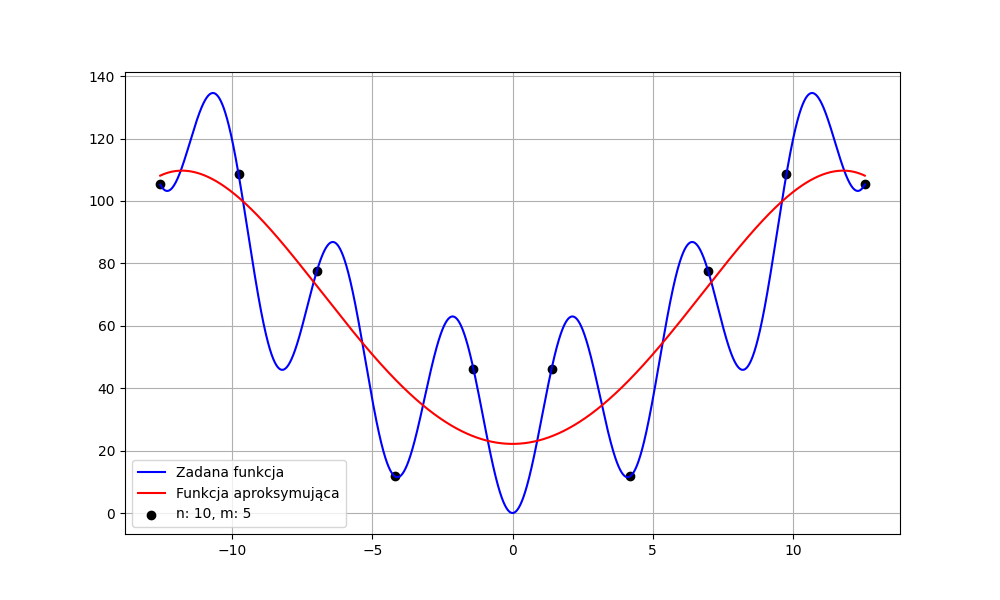
\includegraphics[width=\textwidth]{img26_n=10_m=5.png}
    \caption{Dobre przybliżenie dla 10 węzłów i wielomianu 5 stopnia}
  \end{minipage}
\end{figure}

\newpage

Jak widać na poniższym wykresie ponad dwukrotne zwiększenie liczby węzłów niemal nie poprawiło aproksymacji, z uwagi na niefortunne ułożenie węzłów. Zatem z uwagi na specyfikę funkcji ilość wężłów musi być naprawdę duża.

\begin{figure}[H]
\centering
  \begin{minipage}[b]{0.49\textwidth}
    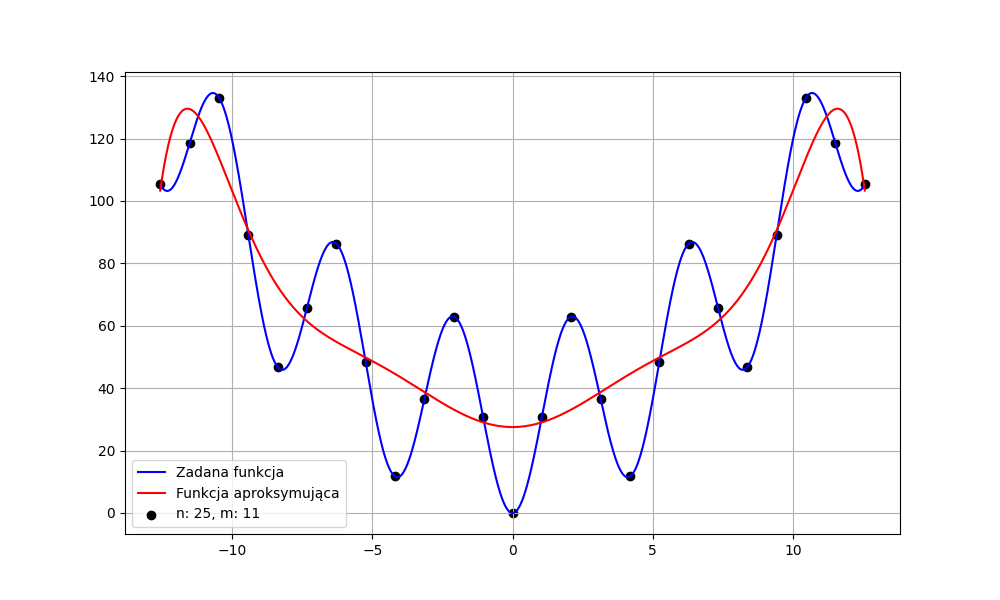
\includegraphics[width=\textwidth]{img27_n=25_m=11.png}
    \caption{Aproksymacja dla 25 węzłów i wielomianu 11 stopnia}
  \end{minipage}
\end{figure}

\subsubsection{Najlepsze otrzymane przybliżenie}

Najlepsze przybliżenie otrzymałem dla 94 węzłów i 25 stopnia wielomianu. Jak widać, ze względu na specyfikę funkcji liczba węzłów musiałą być naprawdę duża, żeby uzyskać dobre przybliżenie.

\begin{figure}[H]
\centering
  \begin{minipage}[b]{0.49\textwidth}
    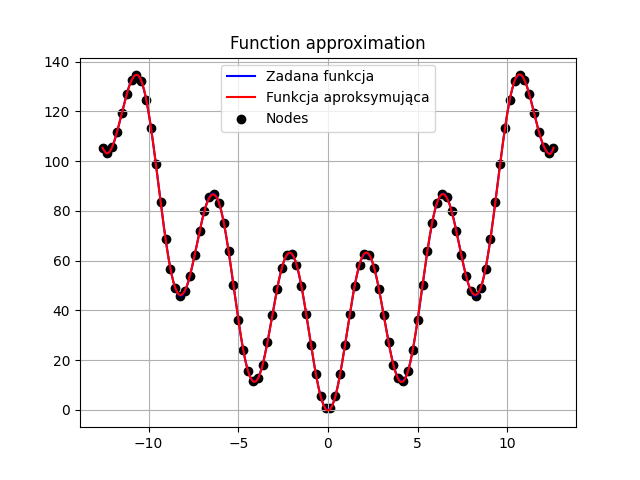
\includegraphics[width=\textwidth]{img28.png}
    \caption{Najlepsze przybliżenie ze względu na błąd maksymalny i średniokwadratowy}
  \end{minipage}
\end{figure}

W poniższe tabeli znajdują się wartości błędów dla powyższego wykresu.

\begin{table}[!ht]
    \centering
    \begin{tabular}{|l|l|}
    \hline
        Błąd maksymalny & 0.5014720569615605 \\ \hline
        Błąd średniokwadratowy & 0.0017181768299556364 \\ \hline
    \end{tabular}
    \caption{Wartości błędów}
\end{table}

\newpage

\subsection{Aproksymacja średniokwadratowa wielomianami trygonometrycznymi}

\subsubsection{Opis teoretyczny}

Ogólny wzór na przybliżenie aproksymacyjne

\[F(x) = c_o\phi_o(x) + c_1\phi_1(x) + ... + c_m\phi_m(x) = \Sigma_{i=0}^{m}c_i\phi_i(x)\]

\noindent
W tym przypadku za funkcje bazowy przyjmuję
\[(\phi_i(x)) = 1, sin(x), cos(x), sin(2x), cos(2x), ..., sin(mx), cos(mx)\]

\noindent
Wzory przybliżające szukaną funkcję wielomianem trygonometrycznym

\[F_m(x) = \frac{1}{2} \cdot a_0 + \Sigma_{j=1}^{m}(a_j \cdot cos(j \cdot x) + b_j \cdot sin(j \cdot x)\]

\[a_j = \frac{2}{n} \cdot \Sigma_{i=0}^{n-1}f(x_i) \cdot cos(j \cdot x_i)\]

\[b_j = \frac{2}{n} \cdot \Sigma_{i=0}^{n-1}f(x_i) \cdot sin(j \cdot x_i)\]

\noindent
Przyjmując n + 1 rónoodległych węzłów aproksymacji opisanych wzorem \(x_i = n \cdot i \cdot \frac{\pi}{2}\), to kolejne elementy bazy będą do siebie ortogonalne i stworzą układ normalny dobrze uwarunkowany.

\noindent
Wielomianami trygonometrycznimi można aproksymować dowolną funkcję okresową, jak wynika z tw. Weierstrassa

\subsubsection{Napotkane Trudności}

Podobnie jak w poprzednich przypadkach niekorzystne ustawienie węzłów w polączeniu z oscylacją funkcji dawało złe przybliżenie, co widać na poniższym wykresie.

\begin{figure}[H]
\centering
  \begin{minipage}[b]{0.49\textwidth}
    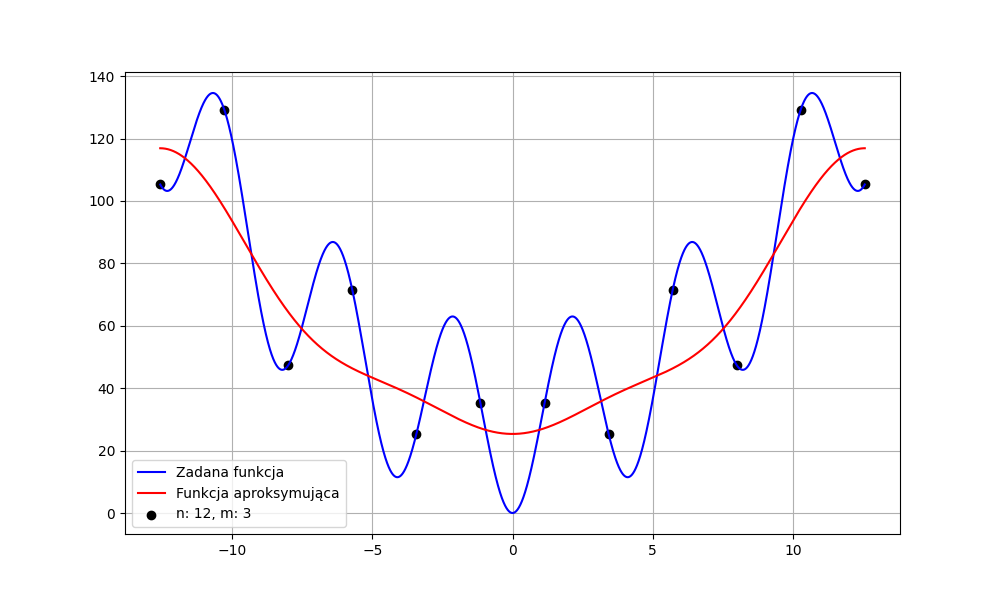
\includegraphics[width=\textwidth]{img29_n=12_m=3.png}
    \caption{Przybliżenie dla 12 węzłów i wielomianu 3 stopnia}
  \end{minipage}
\end{figure}

\newpage

Występowały także trudności z dopasowaniem wielomianu w punktach, gdzie zmienia się monotoniczność, co widać na poniższym wykresie. Największy błąd widać w górnych punktach, a w dolnych przybliżenie jest dobre.

\begin{figure}[H]
\centering
  \begin{minipage}[b]{0.49\textwidth}
    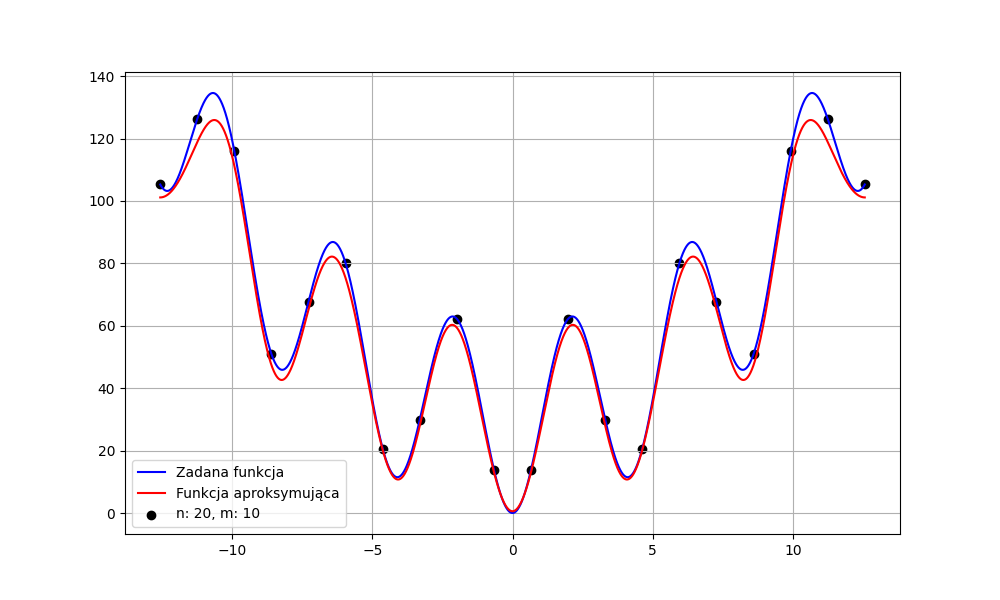
\includegraphics[width=\textwidth]{img29_n=20_m=10.png}
    \caption{Przybliżenie dla 20 węzłów i wielomianu 10 stopnia}
  \end{minipage}
\end{figure}

\subsubsection{Najlepsze otrzymane przybliżenie}

\begin{figure}[H]
\centering
  \begin{minipage}[b]{0.49\textwidth}
    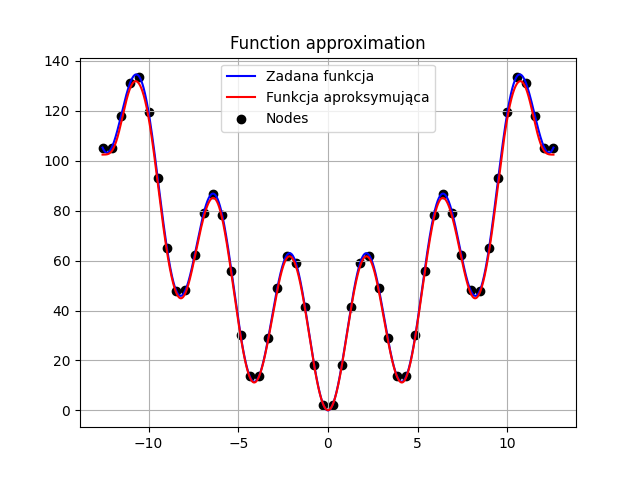
\includegraphics[width=\textwidth]{img30.png}
    \caption{Najlepsze otrzymane przybliżenie}
  \end{minipage}
\end{figure}

W poniższej tabeli znajdują się wartości błędów dla powyższego wykresu.

\begin{table}[!ht]
    \centering
    \begin{tabular}{|l|l|}
    \hline
        Błąd maksymalny & 3.001944813353049 \\ \hline
        Błąd średniokwadratowy & 1.2747973802059938 \\ \hline
    \end{tabular}
    \caption{Wartości błędów}
\end{table}

\newpage

\section{Wnioski}

\begin{itemize}
    \item Największy problemem z zadaną funkcją była jej znaczna oscylacja, co było problemem dla każdej metody przybliżenia funkcji
    \item Drugim najwazniejszym problemem była znaczna zmiana wartości funkcji na krańcach przedziałów, co również powodowało masę błędów przybliżenia na krańcach przedziałów i dochodziło do sytuacji, gdzie w środku przedziału przybliżenie było bardzo dobre, a na krańcach bardzo złe.
    \item Dla każdej metody przybliżenie przy odpowiednio dobranych parametrach jesteśmy w stanie otrzymać zadowalające przybliżenie, jednak w niektórych przypadkach takie przybliżenie może być bardzo niewydajne obliczeniowo.
    \item Nie można jednoznacznie wskazać najlepszej metody przybliżenia, każda z nich ma swoje wady i zalety. Powinna ona  być dobrana do funkcji oraz zastosowania
\end{itemize}


\end{document}